\documentclass[11pt,a4paper]{report}
\usepackage[utf8]{inputenc}
\usepackage[numbers]{natbib}
\usepackage{hyperref}
\usepackage{graphicx}
\usepackage{datetime}
\usepackage{color}
\usepackage{fancyvrb}
\usepackage{microtype}

%% Nicely format and linebreak URLs in the bibliography (and elsewhere).
\usepackage{url}
%% Define a new 'leo' style for the package that will use a smaller font.
\makeatletter
\def\url@leostyle{%
  \@ifundefined{selectfont}{\def\UrlFont{\sf}}{\def\UrlFont{\small\ttfamily}}}
\makeatother
%% Now actually use the newly defined style.
\urlstyle{leo}

%% Nicer formatting of figure captions.
\usepackage[font=small,format=plain,labelfont=bf,up,textfont=it,up]{caption}

\newcommand{\hi}[1]{{\color{red}\em #1\/}\\}
\newcommand{\todo}[1]{\footnote{{\color{red} {\bf TODO:} #1}}}
\newcommand{\ask}[1]{\footnote{{\color{red} {\bf QUESTION:} #1}}}

\setcounter{secnumdepth}{3}
\newcommand{\subsubsubsection}[1]{\paragraph{#1}\mbox{}\\}

% ------------------------------------------------------------------------------
% Title definitions
% ------------------------------------------------------------------------------
\newcommand{\HRule}[1]{\rule{\linewidth}{#1}}     % Horizontal rule

\makeatletter                                     % Title
\def\printtitle{
    {\centering \@title\par}}
\makeatother

\makeatletter                                     % Author
\def\printauthor{
    {\centering \large \@author}}
\makeatother

% ------------------------------------------------------------------------------
% Metadata
% ------------------------------------------------------------------------------
\title{    
            \large \textbf{\uppercase{Project CS - 1DT054}}\\    % Course info
            \large \textsc{Uppsala University}\\[2.0cm]    % University
            \normalsize \textsc{``Treacherous Talks''}   % Subtitle of the document
             \\[2.0cm]                                  % 2cm spacing
            \HRule{0.5pt} \\                            % Upper rule
            \LARGE \textbf{\uppercase{Product Report}}   % Title
            \HRule{2pt} \\ [0.5cm]                      % Lower rule + 0.5cm spacing
            \normalsize \today                          % Todays date
        }

\author{Dilshod Aliev\\
        Jan Daniel Bothma\\
        Stephan Brandauer\\
        Andre Hilsendeger\\
        Rahim Kadkhodamohammadi\\
        Xinze Lin\\
        Tiina Loukusa\\
        Erik Timan\\
        Sukumar Yethadka\\
        }

\begin{document}

% ------------------------------------------------------------------------------
% Maketitle
% ------------------------------------------------------------------------------
\thispagestyle{empty}                % Remove page numbering on this page

\printtitle
\vfill
\printauthor

\tableofcontents

\abstract{
Treacherous Talks is an implementation of a board game (``Diplomacy'') as a web
service. Technical and functional requirements of the project were defined by
our customer --- Erlang Solutions~\cite{erlsol}.

The report explains the project and takes a look at the requirements.
The technical details of the solutions chosen, are presented and their choices
motivated. The features that make the project interesting,
failure tolerance, scalability and multiple interfaces are highlighted.
To conclude, some of our relative weaknesses are mentioned.
}

\chapter{Introduction}
Diplomacy~\cite{diplomacy} is a board game, invented in the 1950s where the goal
is to try to conquer Europe just before WW I. You come close to this goal by
talking to the other players --- by diplomacy --- and making them your allies.
And you achieve it by attacking them when they do not expect it.

The game is and was commonly played over distance --- starting with playing by
mail, then email and nowadays over pretty web pages with full-blown map
visualization.

The requirements we were faced with asked for an implementation of Diplomacy as 
a web service while providing several interfaces to this service. Scalability
and Failure Tolerance were of high priority. 

Even though a board game is a fun thing to implement, we do think that the most
interesting part of our project is the scalability- and fault tolerance-
engineering.

For more details about the project methodology and 
how we tackled problems during the project, please refer to our course report.

\chapter{System Description}
%\hi{System architecture, how it works.
%This is the core of your report, and is therefore most likely the largest section.}

\section{Requirements}
We received a number of requirements from our customer Erlang Solutions that we
were to include in the project.

\subsection{Diplomacy server}
The requirements on the backend were initially grouped as follows:

\begin{itemize}
\item Authentication --- Only registered users should have access.
\item Game master --- To moderate games.
\item Rule engine --- The rule engine should evaluate orders and determine
      the results.
\item Database --- For storing game and user data
\item AI --- Artificial intelligence based player for testing and playing games
      when real players are unavailable.
\end{itemize}

The authentication, rule engine and database features were directly
implemented. The game master role morphed into two roles --- the operator and
the moderator. The AI feature is detailed further below in this section.

\subsection{Three Interfaces}
The requirement stated that we have to provide three interfaces that expose
the same functionality to the user (the operator is forced to use the
web~interface). Those interfaces are:\\
\begin{enumerate}
\item {\bf Web interface} ---
  The game should be accessible via a modern web browser {\em and\/} it should
  use WebSocket to communicate with the browser.
\item {\bf XMPP interface} ---
  The game should be accessible via a chat client using text based orders.
\item {\bf SMTP interface} ---
  The game should be accessible via sending of emails using text based orders.
\end{enumerate}

\subsection{Scalability}
The system should be scalable. Scalability in this context refers to horizontal
scaling where the system should be able to handle more load by simply adding
more nodes. No further explanations were provided regarding this feature, but
since we saw it as a challenge we invested a lot of work into it.

\subsection{Fail-Safety}
The system should be highly available. We interpreted this by assuming that we
should handle hardware failure of physical machines. As with scalability, we
might have been able to get away with less work but this feature as well was
too interesting to resist focusing on it.

\subsection{WebSocket}
WebSocket~\cite{websocket} is a tcp-like connection between a browser and a
web server.
Its novelty is that it is not implemented by polling which makes it quite
fast for updates pushed from the server to the client.
WebSocket can be used by javascript to update only parts of the client page
instead of reloading a page and is a great tool to shift computing to the
client side.

The WebSocket feature was mostly an issue because of the tool support (or lack
thereof) we were faced with. More is explained in Sec.~\ref{sec:frontends}.
Otherwise, WebSocket is an amazing technology and will have a great impact
on web development in the future since tool support is increasing.

\subsection{AI}
Writing a simple AI was a requirement which interested us as well. However, we
were stuck in a tradeoff because time was limited: fail-safety+scalability
vs.\ AI players. In combination with our customer, we agreed on focusing on the
performance characteristics and leaving the AI players for future work.

\section{Architecture}
\subsection{Overview}

Our Architecture is divided in three main blocks, the {\em frontends}, the
{\em controller}, and the {\em backends}. In Fig.~\ref{fig:arch} a running
cluster as it could be configured is shown. {\em Server 1} shows a full
configuration as it includes all three frontends, a backend and Riak. Riak, our
database is explained in Sec.~\ref{sec:riak}.
The operator, however, is free to choose to only run a specific selection of
these and can combine them freely, for example as the {\em Server 2} in
Fig.~\ref{fig:arch}.

\begin{figure}[h]
 \centering
 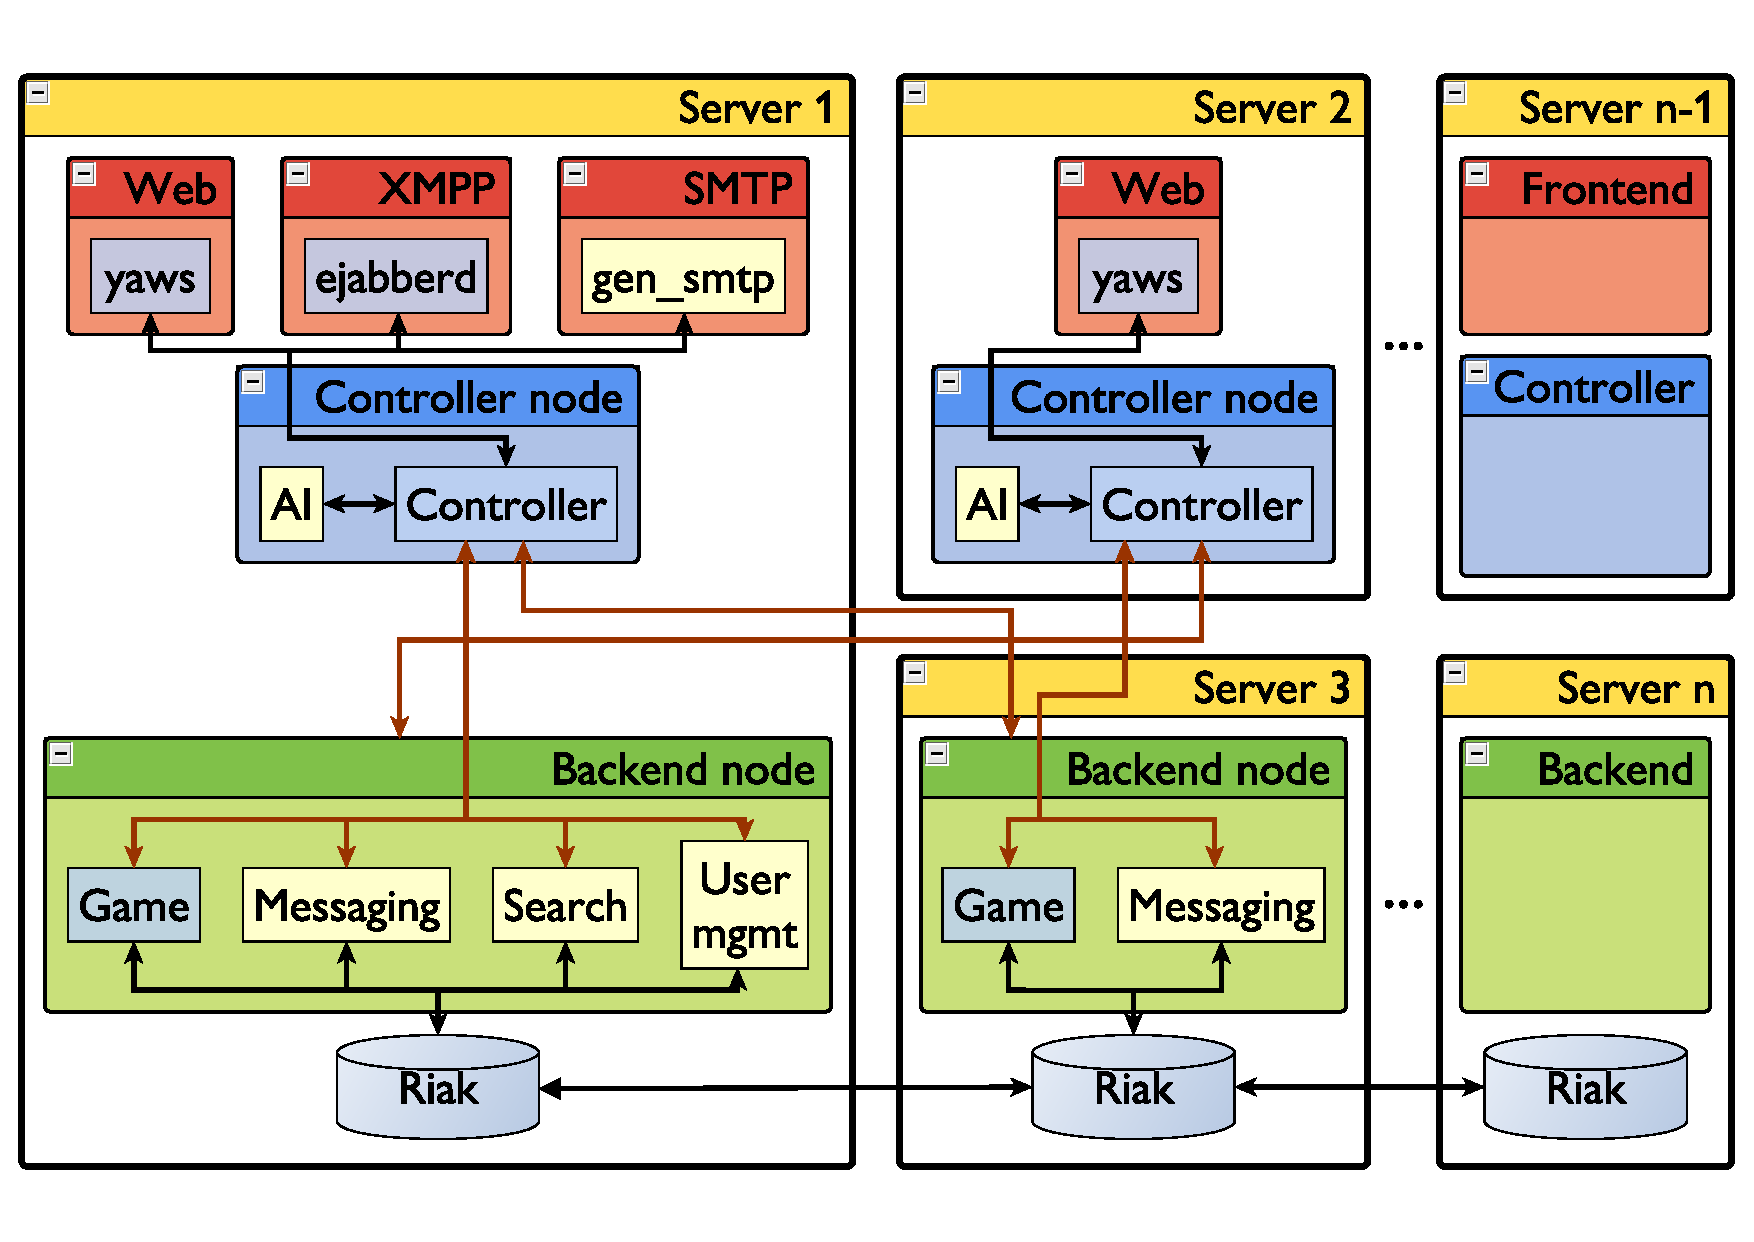
\includegraphics[width=\textwidth]{./graphics/arch.pdf}
 \caption{A possible cluster.}
 \label{fig:arch}
\end{figure}

The responsibilities are not surprising: the frontends receive user input and
transform the input into messages which are sent to the controller.
The controller filters out illegal messages according to the session database
and the user privileges before handing them off to the backends --- which will
respond with an answer.

\subsubsection{Communication between applications}
We follow the MVC\cite{mvc} (Model~View~Controller) Pattern.
The View contains all the supported User Interfaces (Web, SMTP, XMPP). The
Controller is an application that talks to the Model. In the Model there
are backend services (Game, Messaging and User Management) and the database.
Some of the backend services talk to each other, while others work completely
independent. Each box in Fig.~\ref{fig:mod_conn} is an OTP~\cite{erlang_otp}
application, and each of them can be distributed onto multiple nodes and work
simultaneously. The system is database-driven, that is, the backend services are
stateless (see~\ref{sec:stateless}), and any request can be handled
by any node where that service application is running. The communication between
the applications is shown in Fig.~\ref{fig:mod_conn}

\begin{figure}[h]
 \centering
 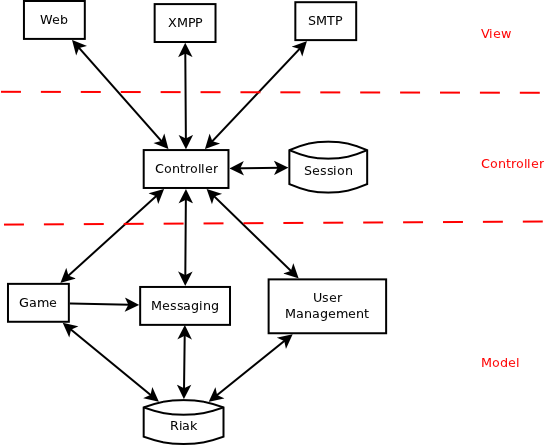
\includegraphics[width=12cm]{./graphics/Modules_Communication.png}
 \caption{Communication between applications.}
 \label{fig:mod_conn}
\end{figure}

Arrows in Fig.~\ref{fig:mod_conn} represent messages, where one application
sends a message to another one. Instead of direct message-passing between
applications, an application calls a function in the API module of the target
application, which sends a message to a worker process in the target application.
The worker process is chosen from the process group for workers
(see Fig.~\ref{fig:service_app}) in that service application. In
Fig.~\ref{fig:mod_conn} you can see two databases. The one in the bottom, Riak
(see~\ref{sec:riak}), is the main database. The other one, Session
(see Mnesia~\ref{sec:mnesia}), is part of the controller and stores sessions.

\subsubsection{Modularity --- and its Relation to Scalability}
One thing that is not immediately visible in our architecture (see Fig.~\ref{fig:arch})
is the fact that the individual applications are very independent of each other. Even
though the architecture graphic shows a complete example of a running cluster,
we can choose to run some applications alone.

If we would, for example, find out that our system is slow because the
web~frontend is the bottleneck, we could add more servers to the cluster that
run only a web~frontend (see Fig.~\ref{fig:arch}, ``Server n-1'').
We can do the same with each of the frontend types, with backends and with Riak nodes.
Our architecture, therefore, inherently supports scaling out very well.

The controller application can be on any physical machine and any node. At least
one instance of the controller application must be running. Extra instances will
set up local copies of the session database, and session processes are distributed
among the instances. We decided to run it on each backend node, since sessions
would be created on the node where the controller worker process handling the
login attempt is running. That distributes work evenly between backend nodes,
except if some local application cannot deal with the request, and this was
found to work as expected during load tests of various cluster sizes
(see Sec.\ref{load_testing_balancing}.

Since the frontends are independent from each other, we did not expect issues
scaling with additional frontends. We therefore focused on testing the performance
of our backends and Riak nodes, as shown in Sec.~\ref{load_tests}.

\subsubsection{Process groups}
\label{sec:process_groups}
The system uses process groups~\cite{process_groups} to provide load balancing by
distributing work across nodes.
This is done by each process in the backend joining the process group for its
application. A calling process can then use the process groups to find a
process to call. The selection is done semi-randomly. Since process groups are
visible globally, if there is not a local process to call, a random process on
another node is used out of that group.
Work is then distributed across other running nodes, providing redundancy. Since
selection is done randomly, it does not guarantee equal distribution between local
or remote processes, but load testing showed this to work sufficiently
(see~\ref{load_tests}).

\subsubsection{Stateless design}
\label{sec:stateless}
One of the ways to scale a system is to use a shared nothing (SN)
architecture~\cite{sn_arch}
where every node is self-sufficient and the system has no single bottleneck.
This allows for a distributed system that is both scalable and fault tolerant.
The implementation of a SN architecture adds a constraint that individual
nodes can only have state that could be lost or must be stateless.

With this in mind, our architecture was designed to allow applications to
be distributed across the physical machines in various configurations
(see Fig.~\ref{fig:arch}). All the system state is moved to the database
and nodes that have state can be restored from the database, in
the event of failure.

We did have to use state in certain parts of the system due to the
distributed nature of the application. Briefly, the parts of the system
with state and the reasoning behind them are:

\begin{itemize}
\item Game timer --- A game has various events associated with it and
tracking these events with time needs a process with a certain amount
of state.
\item Game join process --- Requests from multiple users joining the same
game needs to be serialized to avoid concurrency issues.
\item User session --- Multiple requests from the same user needs to be
ordered since without the ordering the requests can arrive at the backend
at different times creating inconsistent data.
\end{itemize}

\subsection{Frontends}
\label{sec:frontends}
The frontends speak almost the same language to the user, which made the
implementation of front-end logic very generic.

\subsubsection{Web}
The web frontend is running Yaws~\cite{yaws} as a web server.
We initially decided to use Nitrogen~\cite{nitrogen} as a web framework,
but had to drop Nitrogen because of the requirement of using WebSocket for
interaction with the server. Yaws is configured as a ``/" application
module (appmod) so that we can have a single entry point for handling all the
requests. Server side includes (ssi) are also used to load static content via
AJAX~\cite{ajax}.

The web frontend relies heavily on JavaScript~\cite{javascript} since it contains
a large amount of the logic handling user interactions, requests and responses
to the server and gameplay support for the user. We use the JavaScript library
jQuery~\cite{jquery} to update the DOM elements and make AJAX requests.

We use the toolkit Bootstrap~\cite{bootstrap} for the user interface which
allows us to quickly develop web pages. Bootstrap includes basic CSS and HTML for
typography, forms, buttons, tables, grids, navigation, and more. Using Bootstrap
reduced the time needed for web development, allowing us to focus on the
backend.

We had the option of extending Nitrogen to support WebSocket, but after
investigating how much work would be involved, we came to the conclusion that it
would not be feasible given our time constraints. Nitrogen uses
SimpleBridge~\cite{simple_bridge} which provides a standardized interface to all
its supported web servers. We found that adding WebSocket support would mean
adding and changing a lot of code in a lot of places, because of the way
Nitrogen/SimpleBridge is structured. Instead we implemented the web frontend
ourselves with HTML and JavaScript directly served by Yaws.

Throughout the course of the project the WebSocket protocol has
been under development. Only towards the end of the project has a protocol
(RFC 6455) been released that has been proposed to be the official standard.
Since the protocol might have changed significantly during the project, we
decided to commit to a particular WebSocket draft version, and a web browser and
server version that support it. This gave us a stable base to develop on.

We chose the ``hybi-10'' draft of the protocol~\cite{hybi-10} which was
supported by Chromium 14 and a fork of Yaws 1.91~\cite{yaws-fork}. This draft
version was chosen because it appeared likely to become the basis of the final
standard~\cite{new-websocket-google-blog} while the earlier drafts were
incompatible.

When RFC 6455 was released, only minor changes were needed to make the branch of
Yaws we were using compatible. We now support any browser that implements
the ``hybi-10'' and newer drafts, or RFC 6455.

Yaws has since merged a fork with support for RFC 6455 but we have not updated
our code to use this version of Yaws due to time constraints and instead still
use our fork of Yaws 1.91~\cite{our-yaws}.


\subsubsection{XMPP}
Using ejabberd~\cite{ejabberd} as XMPP server was an obvious choice since ejabberd is the
standard solution for XMPP servers and ejabberd is implemented
in Erlang which led us to hope that it would play well with our code.

There are three ways to implement integration with ejabberd:

\begin{itemize}
\item Client --- A bot that uses an Erlang client such as exmpp~\cite{exmpp} can be used to
connect to the server.
All users send messages to the bot via the ejabberd server. e.g. bot@example.com.
An issue the jabber client has, is that it doesn’t scale. Using a single bot
will mean all the users will have to be in the bot’s roster (user list).
Ejabberd doesn’t handle the scaling of rosters very well (known to fail for
$>$ 40k clients~\cite{40k-roster}).

\item Component --- A component is a trusted piece of an XMPP server that can send
and receive arbitrary stanzas.
In other words, we can add a module to ejabberd and define a virtual domain to
get all messages that are sent to this domain.
Because the name of a component is a domain (example: tt.localhost), a component
can pretend to be many users.
Any stanza addressed to service@tt.localhost will be delivered to tt.localhost
no matter what the value is of 'service'.
\item S2S (server to server) --- This is the next step for those who need very
large scale. This was not suitable for us since it requires us to learn a new
protocol and is most possibly not necessary for our needs.
\end{itemize}

We decided to use component to communicate with users. We added a module to
ejabberd that registers a hook to get all the messages that are sent to
tt.localhost and forwards it to our backend. Ejabberd automatically spawns a
new process for a new user who sends messages to this component.
If we need to communicate with a user, we use the corresponding process.

In this way, not only users that have an account on our ejabberd server, but
also users that have account on any XMPP server can send their commands to the
specified address and use our system.

\subsubsection{SMTP}
SMTP, together with POP and IMAP are the three most prevalent protocols for
today's email servers.
SMTP is used for sending emails from clients to servers while POP or IMAP
are used for retrieving email from servers to clients.
For our email server, we found three qualified candidates: Erlmail~\cite{erlmail},
gen\_smtp~\cite{gen_smtp} and erlang-smtp~\cite{erlang-smtp}.
At first sight, Erlmail seemed to be the most competitive one since it
supports all these three protocols when others support only one or two of them.
However, since our SMTP frontend doesn't directly talk to email clients, we
figured out that there's no need for an email retrieving mechanism for our
servers. Therefore, we picked gen\_smtp server as our SMTP frontend since all
of its modules are only focused on SMTP. In our system architecture, the
SMTP~frontend is the bridge between the client side and the backend
(see Fig.~\ref{fig:smtp_arch}).
Once the SMTP frontend receives an email from the client side, it will extract
the email content and pass it to the backend controller. The controller will
interpret and execute the valid orders carried by the email content, then
respond to client side through the SMTP frontend again.

\begin{figure}[h]
 \centering
 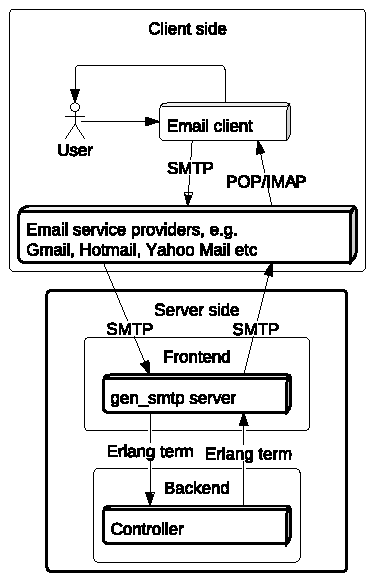
\includegraphics[width=8cm]{./graphics/smtp_arch.pdf}
 \caption{SMTP communication between client side and backend.}
 \label{fig:smtp_arch}
\end{figure}

\subsection{Controller}
The main characteristic distinguishing requests is whether they belong to a
session or not.
So the controller has two kinds of workers.
Those responsible for requests with a session and those for requests without.

\begin{figure}[h]
 \centering
 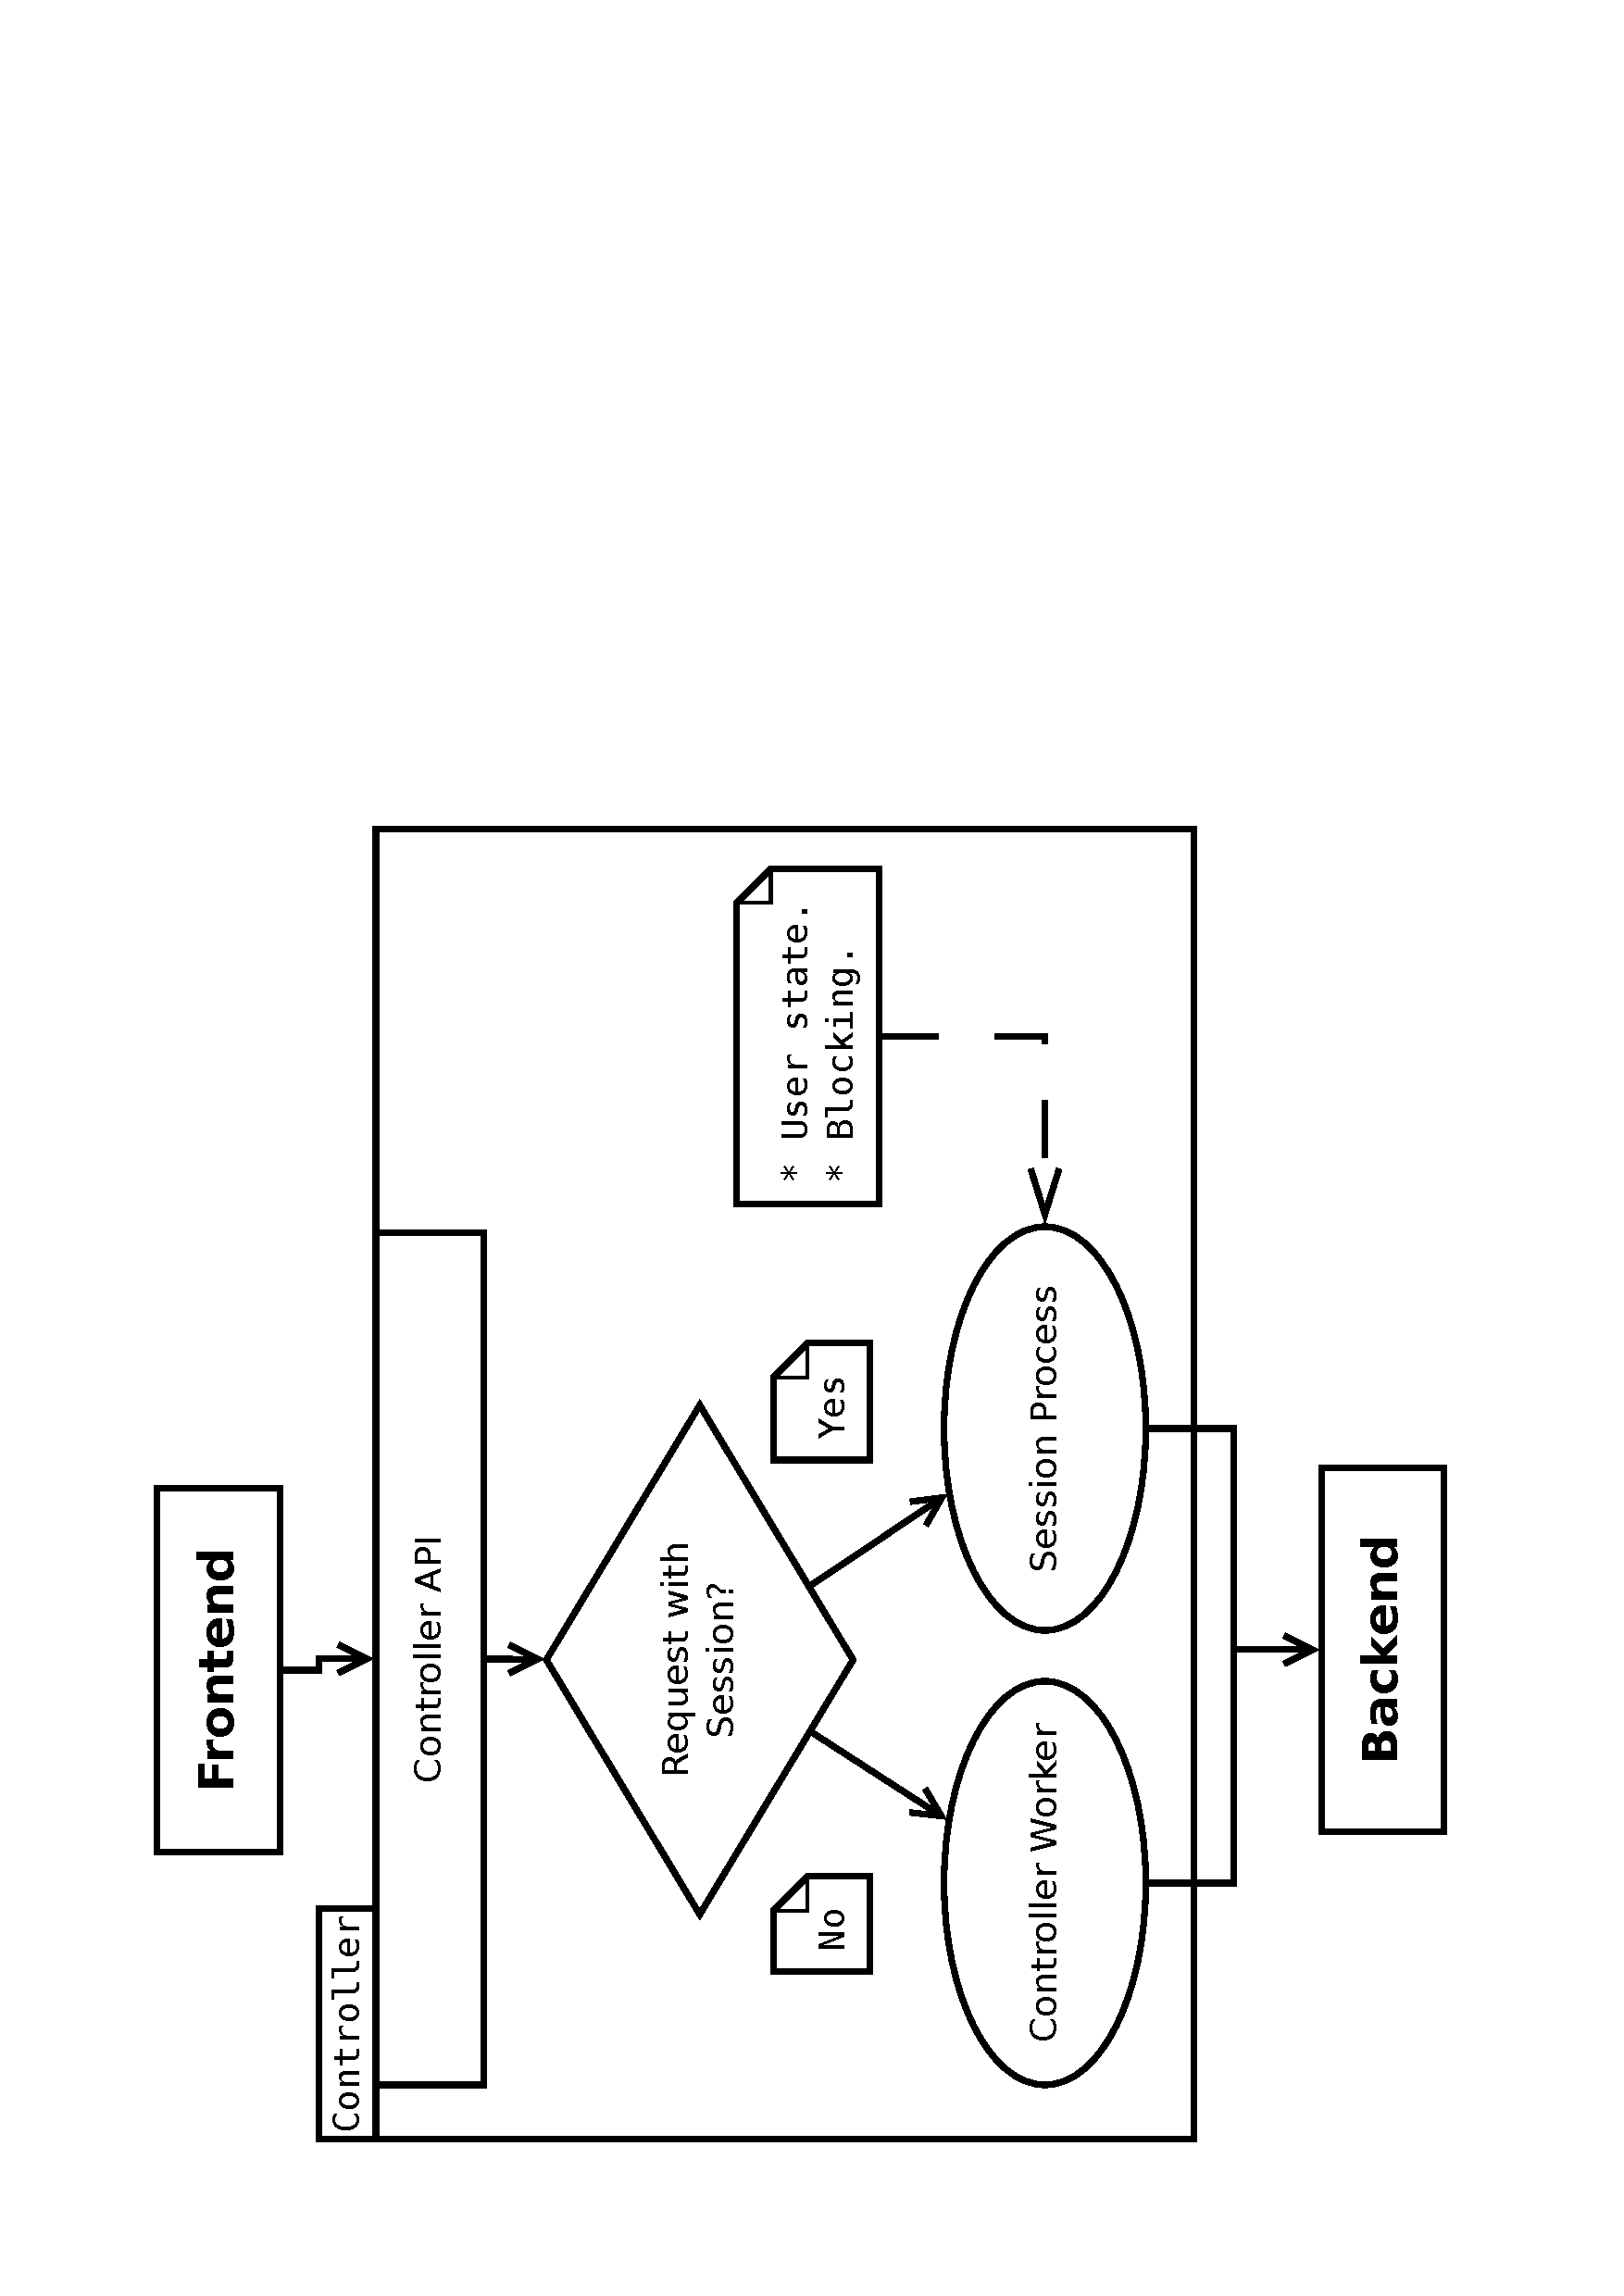
\includegraphics[width=13cm, angle=-90]{./graphics/Concurrency_-_session_proc.pdf}
 \vspace{-1cm}
 \caption{Controller flow of a request with/without session.}
 \label{fig:controller:session_proc}
\end{figure}

The simple ones without sessions are completely stateless and can handle
requests from any user.
A fixed number of them is spawned on startup and will handle requests on
arrival.
Their main responsibilities are registration, login and the like.
Fig.~\ref{fig:controller:session_proc} illustrates this.

\subsubsection{Session Management}
\label{sec:session}
The session management consists of a group of processes and a Mnesia table.
Each session spawns its own session process and writes an entry into the Mnesia
table, so that one such process exists for each logged in user.
The Mnesia table is necessary to have a mapping between users and sessions.
The processes handle all requests for their session and have the session data
(user data, knowledge of how to push events to the frontend, etc).
The reasons for that are concurrency issues
(more on that in~\ref{sec:concurrency}).


\subsubsection{Access Control}
Which users can perform which actions on the system is defined by a set of
identities known as roles. The system has four roles:

\begin{itemize}
\item User --- A registered member of the system who can create and play games.
\item Blacklisted user --- A user who has been removed from the system.
\item Moderator --- A user with enhanced privileges to moderate games and help
other users.
\item Operator --- An administrator who has complete control over the system.

\end{itemize}


\subsection{Riak}
\label{sec:riak}
The choice of Riak~\cite{riak} as database was a careful one: we evaluated Riak,
couchDB~\cite{couchdb} and Mnesia~\cite{mnesia} but Riak was our favourite in the
end --- its scalability features are very simple to use and its potential for
scalability is what we needed. Due to consistency issues, we had to resort to
using Mnesia for sessions (see~\ref{sec:stateless},~\ref{sec:session}) and the game joining
processes (see~\ref{sec:stateless}), as it provides transactions.

Riak proved to be a good choice for us since its performance parameters (called
``CAP controls''~\cite{cap_controls} in riak-lingo) are very easy to tune and it
is quite well documented how Riak behaves under load. The scalability problems
we had came from using the search module too much
(see~\ref{sec:load_tests:key_filtering}).

Riak is a distributed key/value store that connects an arbitrary number of
{\em nodes} to form a cluster. All of these nodes can --- but don't have to ---
run on different machines (and do so in our standard setup). As soon as one
node receives a write for one key/value pair, the node will make sure that the
data is written on a certain number of nodes. That number can be chosen from
$[1 \ldots N]$ where $N$ is the number of nodes.
No node in a Riak cluster is privileged, they all have exactly the same
responsibilities which makes the architecture simpler.
The ease of adding nodes to a running Riak cluster is one of its main
advantages, data are redistributed in order to achieve fair distribution after
one node is added. This can, of course, have performance implications but they
were not measured by us (see~\ref{load_tests}).

\subsubsection{eLevelDB}
Riak's storage backend was a problem. Riak has the feature to switch the
storage backend --- the way, key/value pairs are stored on a node.
We initially used {\tt eLevelDB}~\cite{eleveldb} because it supported secondary indices, a
feature we wanted. However, {\tt eLevelDB} showed degrading performance
in our context: the throughput of database operations was decreasing linearly
over time, down to zero. We could not pinpoint the problem, so we had to switch
the storage backend to {\tt bitcask}~\cite{bitcask}, Riak's standard storage backend.
Bitcask does not support secondary
indices~\cite{secondary_idx}\cite{secondary_idx_riak},
and because of that it was necessary to use
{\tt riak\_search} more --- which led to scalability
issues (see~\ref{sec:load_tests:key_filtering}).

\subsubsection{Mnesia}
\label{sec:mnesia}
A user can access our system from multiple frontends resulting in
concurrency issues. We dealt with them by making sure that the user
can use only one frontend at a time.

Another issue was that multiple orders sent by the same user can arrive at the
backend in a different sequence, thereby creating inconsistent data. This was
fixed by serializing the user's commands.

The implementation of the above two solutions is not possible using Riak since
it is an eventually consistent~\cite{eventual_consistency} database.
Mnesia, which is distributed and has transactions, is the right fit.

We use Mnesia to keep track of user sessions. Combining this with
the use of one Erlang process per session makes the implementation complete.


\subsection{Backend}
\subsubsection{Game Managing}
Managing games is split up in two main tasks: {\em game timing\/} and
{\em order-processing}.

Game timing is implemented as a {\tt gen\_fsm} that changes states when a game
phase needs to stop, eg.\ when the deadline for handing in orders is over.

Before a phase is started, the rules processing is done by a module we call
the ``rule engine'': the orders which were sent by the users before the
deadline are read from the database and passed, along with the current game
map, to the rule engine.
\subsubsection{Messaging}
Since communication is very important in the game --- some even say, that the
game is mostly about communication --- the messaging module is a very central
feature for us. We support two types of messages: {\em in-game\/} and
{\em off-game\/}-messages.

In-game messages never involve the user nickname for tactical reasons: if someone
remembers my nickname, he/she has an easier time to anticipate my moves since he/she
will likely remember my actions in previous games.
Or, worse: he might still hold a grudge against me. This is why you never
communicate with players in-game by using their nickname, but by using their
country.

Off-game messages on the other hand are sent to a nickname and the recipient
will see the sender's nickname. The basic use case for the off-game messaging
is giving users the chance to set up games for their friends and tell them
about it.
\subsubsection{Search}
Our search module provides the functionality to search, for instance, for
games, based on their properties (like all game parameters). For the
implementation of search, we relied on the Riak extension {\tt riak\_search}.

Riak search is a search engine that is tightly coupled with the Riak datastore.
We added a precommit hook so that whenever a new object is added or an old one
updated, the object is indexed (tokenization with standard Lucene analyzers)
and saved.

Riak provides a rich query language consisting of term searches, field searches,
boolean operators and wildcards to fetch matching objects ordered by relevance.

This feature comes with a price though and should be used with caution.
During load testing we discovered, that it should be avoided for often updated
data.
As it has to re-index all fields of an object on every write it can kill the
performance.
Therefore we tried minimizing writes on search indexed data and if possible not
to use the Riak search feature at all.

\subsubsection{User Management}
The user management module's purpose is to create, update, read, delete users
in or from the database. The implementation is quite short and should contain
few surprises.

\subsection{Concurrency}
% http://redmine.pcs/projects/dip/wiki/Concurrency_handling
\label{sec:concurrency}
\subsubsection{Problem}
Handling concurrency can be quite tricky.
Especially with an eventually consistent database like Riak.
The system is designed so that any node can handle incoming requests,
since it is database driven, and on one node there are multiple workers,
that can perform the same tasks.
Thus two requests involving an update on the same key-value pair can, and will,
end up on different workers or even nodes.
This can lead to inconsistency, because they might have different work load
and execute the tasks out of order.
Fig.~\ref{fig:concurrency:problem_expl} illustrates this.
\begin{figure}[htbp!]
 \centering
 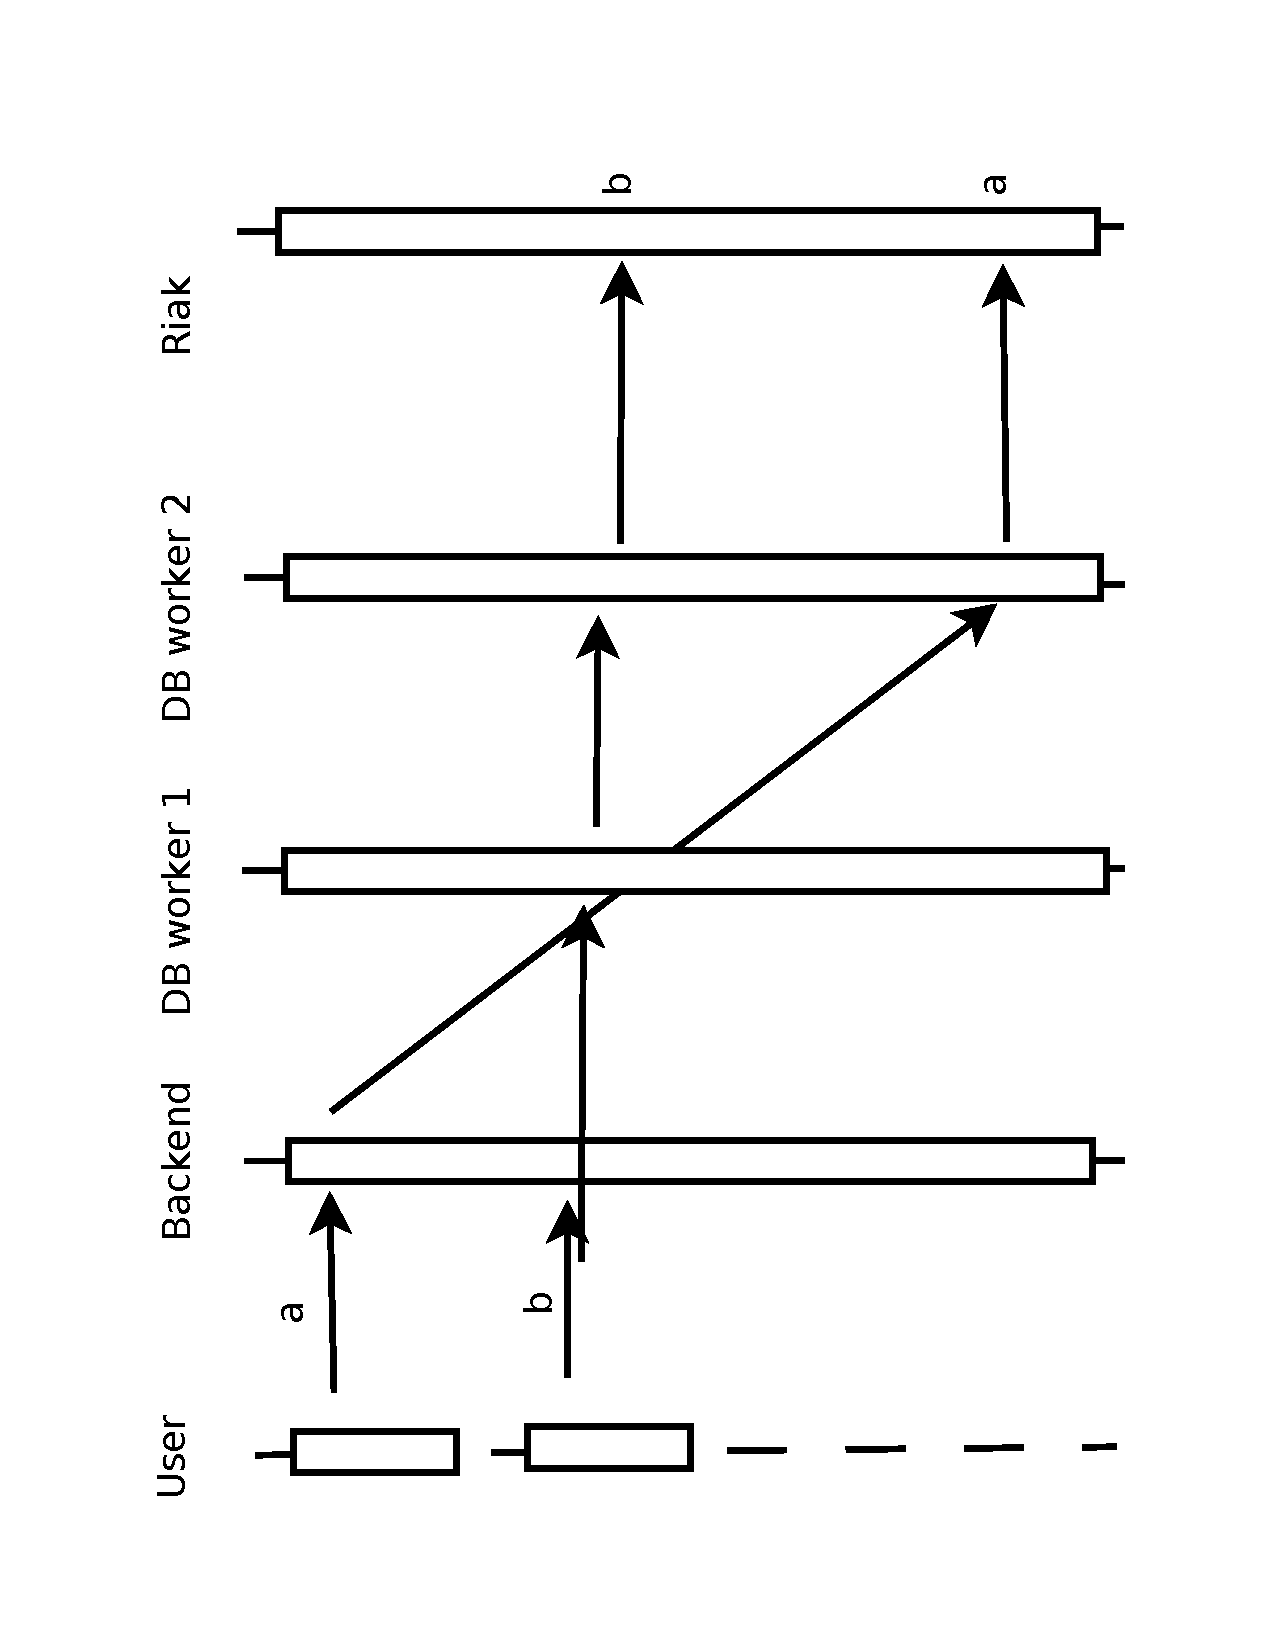
\includegraphics[width=10cm, angle=-90]{./graphics/Concurrency_-_Earlier_session_write_replace_later_session_write.pdf}
 \vspace{-1cm}
 \caption{First request written after second one, leading to inconsistency.}
 \label{fig:concurrency:problem_expl}
\end{figure}

\begin{figure}[htbp!]
 \hspace{-3cm}
 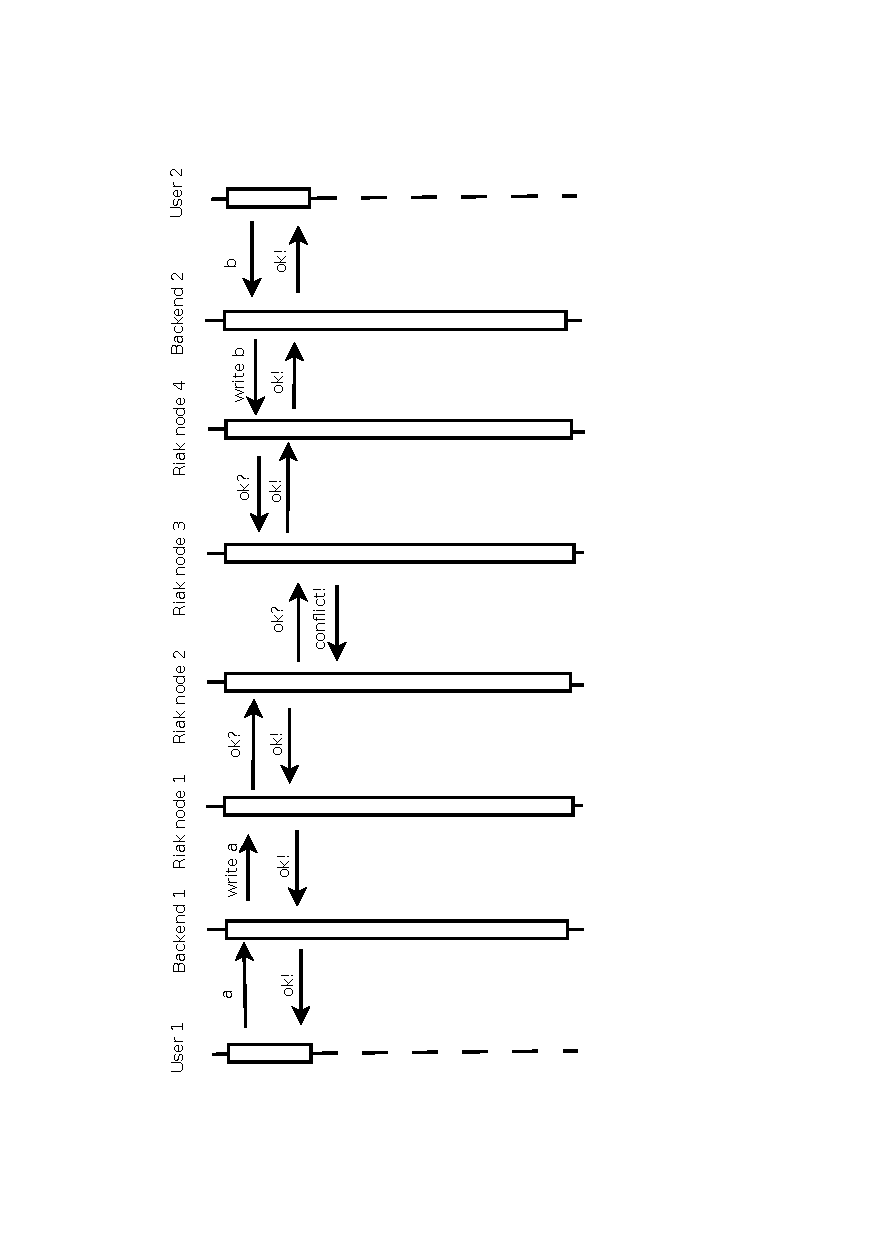
\includegraphics[width=\textwidth, angle=-90]{./graphics/Concurrency_-_Siblings.pdf}
 \vspace{-4cm}
 \caption{Sibling creation.}
 \label{fig:concurrency:siblings}
\end{figure}
Another problem is shown in Fig.~\ref{fig:concurrency:siblings}.
Two different nodes might end up writing to the same key without even knowing
there was a concurrent write.
Riak's CAP control specifies how many Riak nodes should respond a positive write
before returning.
In case 2/4 have to respond, two different writes can get the ``ok''.
Our backends would not even know there was a simultaneous write.
Riak tries to automatically resolve this among others with vclocks~\cite{vclock}.
If Riak cannot resolve this it will leave both values as so called siblings
in the database.
It is then up to the backend to resolve the conflict on the next read
and write back the value which was decided to be the value that resulted after
the conflict resolution.

\subsubsection{Solution}
A common solution for this problem is to serialize requests/writes to the same
key.
A sequential execution of tasks will always ensure the correct order and not
create inconsistent data.
In Erlang this is best done with processes.
Each process has a message queue and can only handle one message after another.
Thus requests are serialized if they have to go to the same process and if they are
all matched against the same pattern in the receive statement.

In our system there are two kinds of interactions that need to be considered:
single user concurrency and multi user concurrency.

\subsubsubsection{Single user concurrency}
Single user concurrency involves all the data that is written by only one user,
like user profile updates and game orders.
In order to serialize these there is one process for each session,
and each user is only allowed to be logged in once at a time.
\begin{figure}[htbp!]
  \centering
 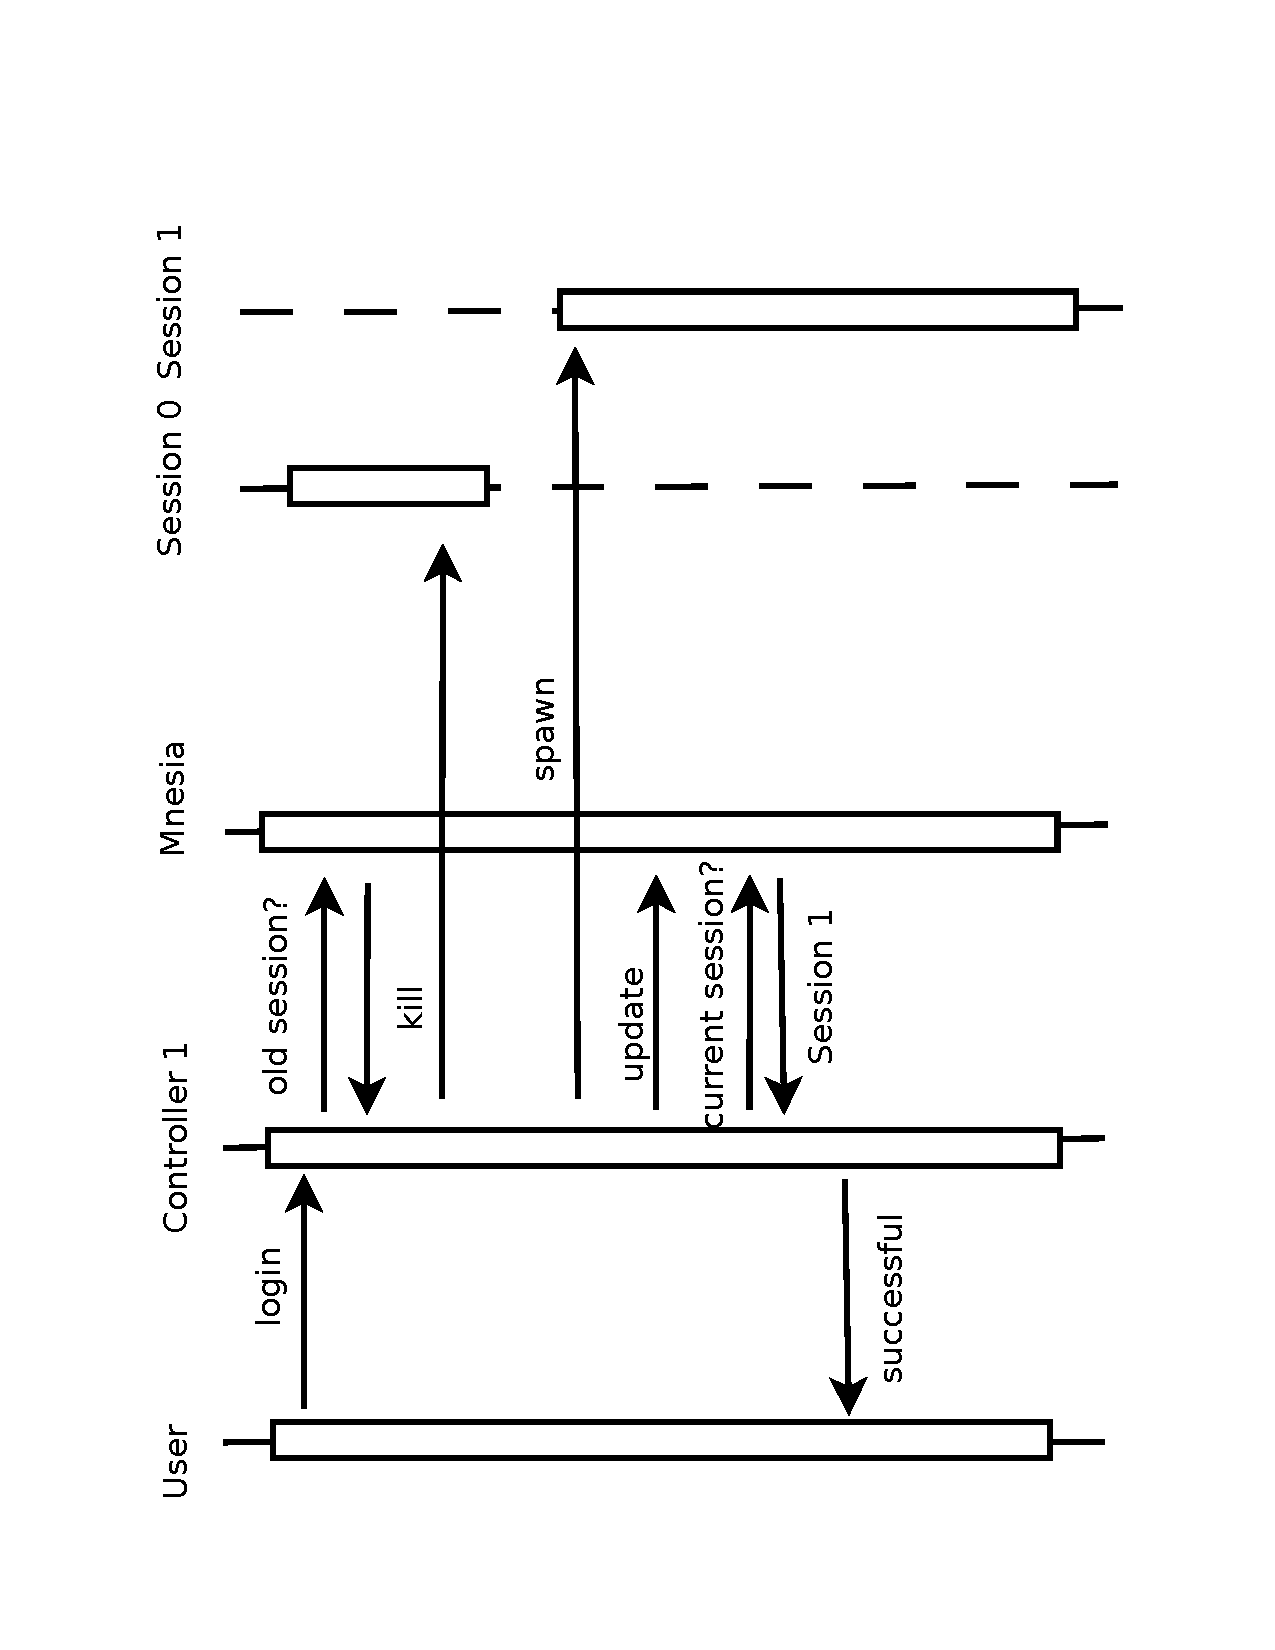
\includegraphics[width=11cm, angle=-90]{./graphics/Concurrency_-_Login.pdf}
 \vspace{-1cm}
 \caption{User login.}
 \label{fig:concurrency:login}
\end{figure}
To ensure only one active session the login has to consider concurrency as well.
Fig.~\ref{fig:concurrency:login} shows how the login works.
Any old session needs be terminated before we can start a new one.
Also, we use Mnesia instead of Riak to store session information,
as it supports transactions.

Unfortunately this still leaves one case.
For example a user might re-login while his requests to update the profile is
being handled and then tries to update the profile again before the previous
update has been written.
This is very unlikely to happen, as the user needs to do the update very
quickly.
However it still needs to be handled.
\begin{figure}[htbp!]
  \centering
 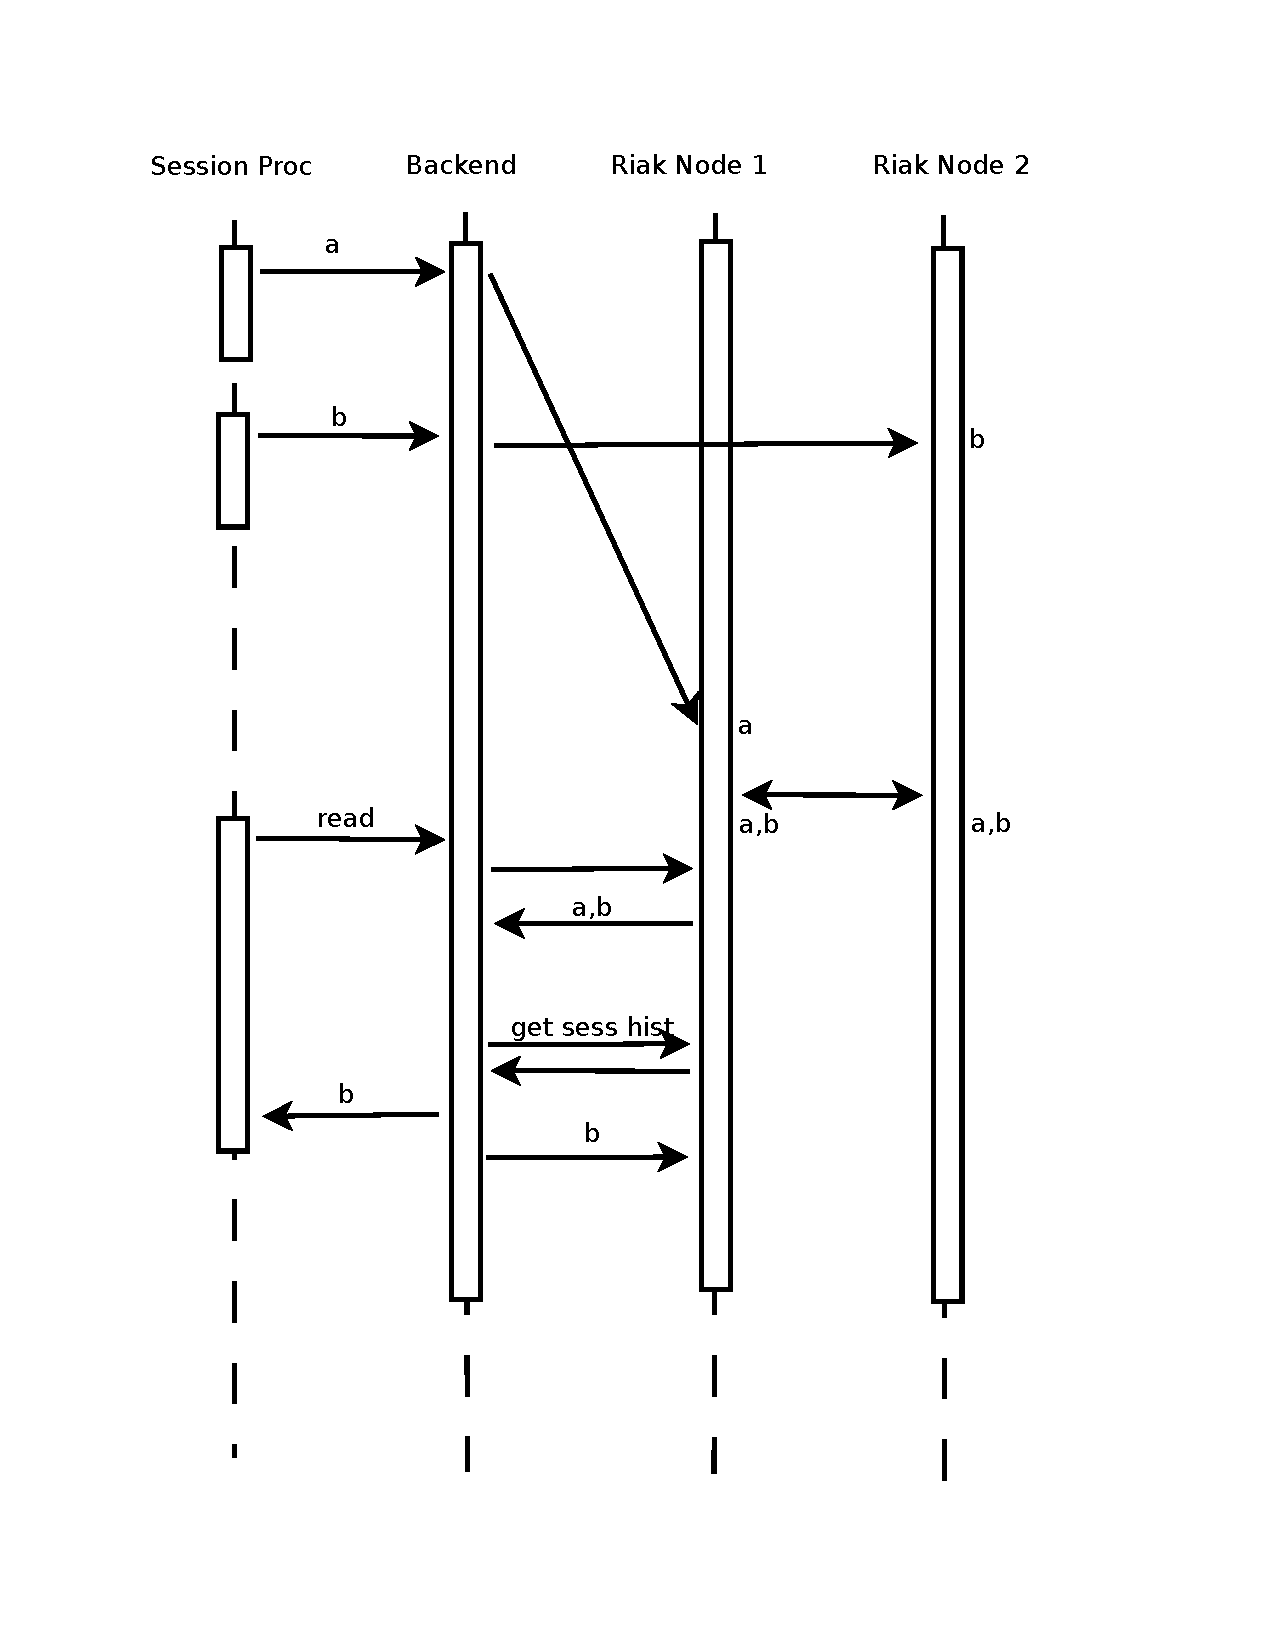
\includegraphics[width=13cm]{./graphics/Concurrency_-_Conflict_resolution_using_session_history.pdf}
 \vspace{-1cm}
 \caption{Siblings resolutions using session history.}
 \label{fig:concurrency:history}
\end{figure}
We use a session history to resolve siblings, which is updated during login.
Additionally we store which session was responsible for the update.
When the backend encounters siblings it then checks the session history which
is the newer one and picks the corresponding value to be the correct one.
Fig.~\ref{fig:concurrency:history} illustrates this.

\subsubsubsection{Multi user concurrency}
Multi user concurrency involves the data that can be written by multiple users,
like joining or updating a game.
In general we tried to  design our database schema to avoid shared writable data
as much as possible.
For example the game orders for a certain phase could be stored as one value in
Riak, instead we keep one value for each player.
This leads to seven reads on phase change, but order writing does not have
conflicts.

Nevertheless, we could not avoid it in all parts of the system.
Multiple users might try to join the same game.
There might be a conflict if they want to play the same country or only one
spot is left.
Furthermore, the creator of the game is not allowed to update the game once a
player has joined it.
Therefore we have a game joining process for every game that has not started
yet.
All join and update requests go through that process, thus ensuring consistency.
To ensure only one such process per game we use Mnesia due to its transactions.

\section{Code organization}

The project consists of a set of Erlang applications logically grouped
based on their functionalities. We have two more directories at the
project level, one for external tests and the other for the release.
Below is the high level directory structure of the project.

\begin{verbatim}
   |-apps
   |---cluster_manager
   |---controller_app
   |---datatypes
   |---db
   |---game
   |---gen_moves
   |---load_test
   |---message
   |---necromancer
   |---service
   |---smtp_frontend
   |---system_manager
   |---user_management
   |---utils
   |---web_frontend
   |---xmpp_lib
   |-ext_test
   |---bench
   |---fault_tolerance
   |---smtp_integration_test
   |---websocket_client
   |---xmpp_integration_test
   |-rel
\end{verbatim}

A short description of each application can be found in Table~\ref{table1}.

\begin{center}
    \begin{table}[t]
    \centering
    \begin{tabular}{ | l |p{10cm}|}
    \hline
    \textbf{Application} & \textbf{Description} \\ \hline \hline
    cluster\_manager & escript for management of the distributed
    cluster \\ \hline
    controller\_app & The controller application \\ \hline
    datatypes & A central place for common configuration. It contains bucket
    names and records \\ \hline
    db & The database wrapper that handles all the db requests\\ \hline
    game & Contains game logic, game timer, rule engine and other game
    related code \\ \hline
    gen\_moves & Generates moves that can be used for load testing \\ \hline
    load\_test & Code used for load testing \\ \hline
    message & Code used for handling messages \\ \hline
    necromancer & Code used for resurrecting certain processes from dead VMs \\ \hline
    service &  OTP application library that provides functionality used by
    all service applications \\ \hline
    smtp\_frontend & Handles all the mail communication \\ \hline
    system\_manager & Single point of entry for configuring and controlling
    the whole system on a server. \\ \hline
    user\_management & Handles all user related functions \\ \hline
    utils & Commonly used tools and utilities \\ \hline
    web\_frontend & Code for handling the web frontend, including client
    side code \\ \hline
    xmpp\_lib & Library for handling XMPP communication \\ \hline
    \end{tabular}
    \caption{Applications with their short descriptions.}
    \label{table1}
    \end{table}
\end{center}


Additional notes on the code:

\begin{itemize}
\item General Erlang coding style and conventions were followed.
\item The public API of all the modules has specs and edocs.
\end{itemize}


\section{Supervision}
A supervisor in Erlang is a process that supervises processes it has spawned.
The supervisor can spawn new child processes and if one of them would die, it
can act according to its configured restart-policy, for example, it could be
configured to never restart children or alway restart them, independent of the
``cause of death''.

Each application (that is not only a library) in our backend and also the
controller have a supervision tree structure that enables an operator to fine
tune the number of workers of each application, it also makes it possible
to inspect the status of applications on each server.

As seen in Fig.~\ref{fig:service_app}, there is one process group
(see~\ref{sec:process_groups}) for the application workers, and a ``management''
group. The processes in the worker group are the ones doing the heavy work in an
application. The ``manager'' of each application in each node makes it
possible to change the number of workers, it also makes it possible to traverse
the group of managers to be able to get the status of each application on every
node it is running on. The supervisors will always restart its workers if they
die unexpectedly.
\begin{figure}[h]
 \centering
 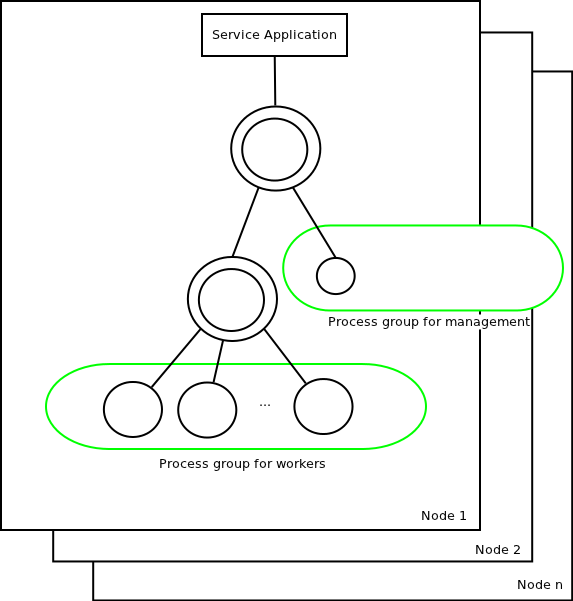
\includegraphics[width=\textwidth]{./graphics/Service_Application.png}
 \caption{General supervision structure for applications, double-rings are
supervisors.}
 \label{fig:service_app}
\end{figure}

The game application's supervision tree is slightly different, as it also has a
number of game timers, which don't belong to a process group as seen in
Fig.~\ref{fig:game_app}. The game timer processes have their own supervisor
which will restart the processes in case the process would die in an unnatural
way, that is if the game has not yet finished nor been stopped by an operator.
\begin{figure}[h]
 \centering
 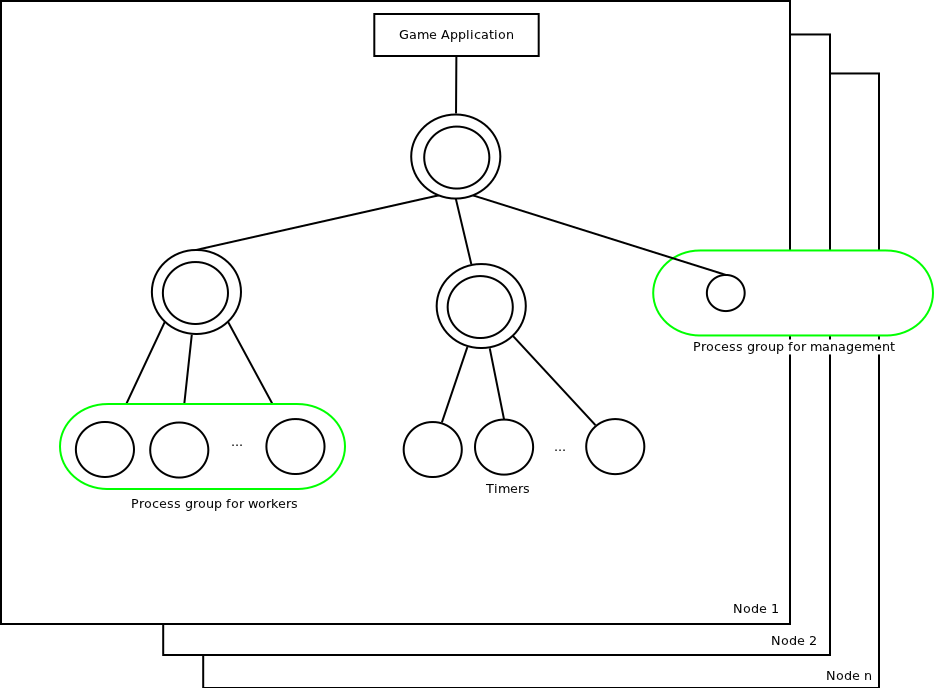
\includegraphics[width=\textwidth]{./graphics/game_Application.png}
 \caption{Supervision tree for the game application.}
 \label{fig:game_app}
\end{figure}

\chapter{Treacherous Talks}
\section{The Three Interfaces}
\subsection{HTTP}
The user goes to the landing page, there he/she finds a link to register which will
display a simple form for him/her to fill out. After the user is registered, he/she is
able to log in using the login textfields on the landing page.

After logging in, the user is shown a dashboard page (see Fig.~\ref{fig:dashboard})
where he is able to search for games, look at the games he is playing in (if
any) and chat with other users in-game or off-game.

\begin{figure}[h]
 \centering
 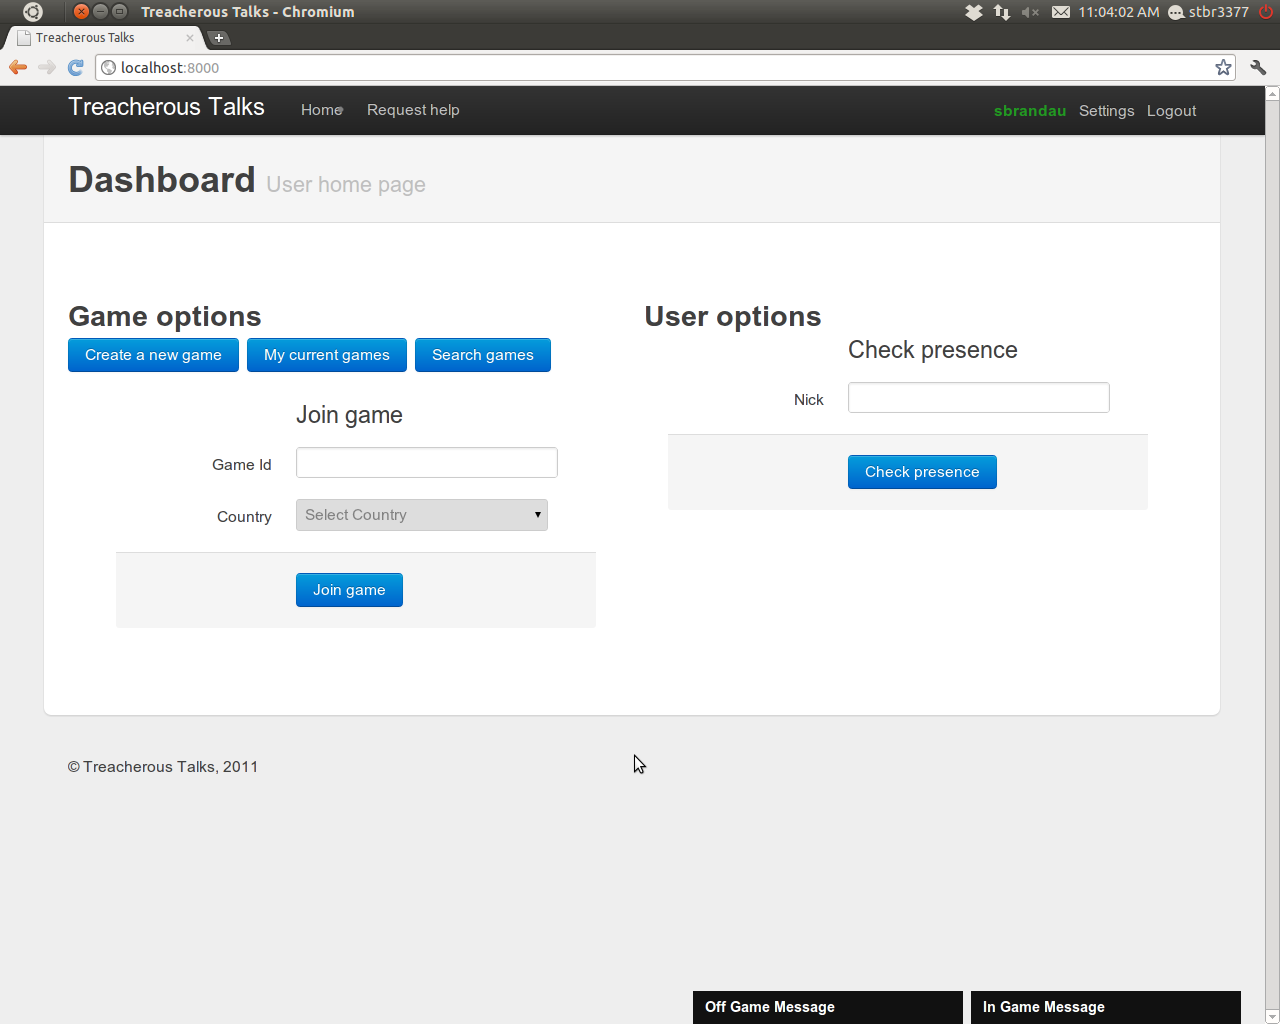
\includegraphics[width=\textwidth]{./graphics/overviewpage.png}
 \caption{The dashboard page.}
 \label{fig:dashboard}
\end{figure}

The web frontend has several key advantages over the two purely text based
frontends:
\begin{itemize}
\item The user does not need to remember his session id.
\item The user sees a graphical map (generated using a HTML5 canvas),
  see Fig.~\ref{fig:map}.
\item It allows users to have a better gaming experience since the graphical map
is interactive. By simply clicking and dragging the pieces on the map,
corresponding orders will be automatically generated, see Fig.~\ref{fig:orders}.
\end{itemize}

\begin{figure}[h]
 \centering
 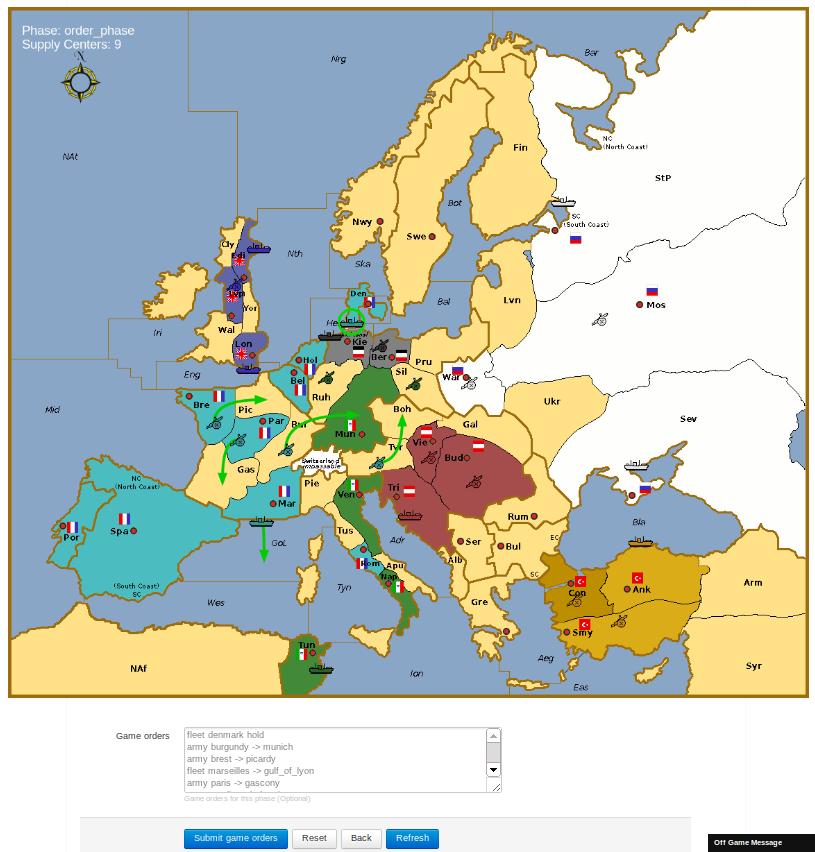
\includegraphics[width=\textwidth]{./graphics/graphicalmap.png}
 \caption{The graphical map.}
 \label{fig:map}
\end{figure}

\begin{figure}[h]
 \centering
 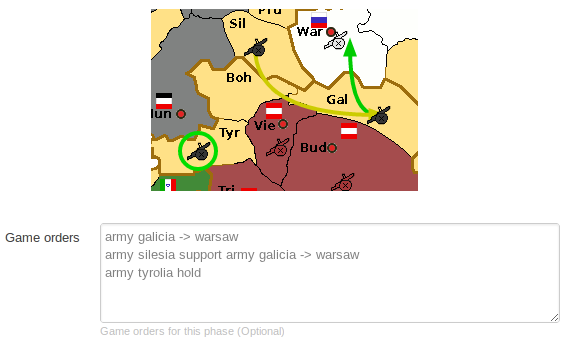
\includegraphics[width=\textwidth]{./graphics/orderssmall.png}
 \caption{The generated orders.}
 \label{fig:orders}
\end{figure}

\subsection{XMPP}
Users who log into our XMPP server, will get the address of the component that
commands should be sent to in an instant message. If a user has an account
on any other XMPP server, they can play the game by sending commands as instant
messages to the server's user. For development, we used the user
``service@tt.localhost'', but this is only accessible from the host where ejabberd
is running. To enable access from other ejabberd servers and connecting from
other hosts, {\tt tt.localhost} in the {\tt tt\_bot} module should be changed to
a domain where ejabberd is configured to listen for connections.

If a user sends  ``HELP'' or any unknown command to our component, it will
return the list of all valid commands. All commands can be found in
appendix~\ref{sec:textbasedcmd}.
Each command starts with the command keyword and must end with the ``END'' tag.
If the user enters some text before the command keyword or after the end
keyword, they are simply ignored. Users can get the list of all mandatory fields
for each command by sending the command name and ``END''.

The user will get a unique session ID after logging in. The session ID should be
stored, because it is necessary for all the future commands.

\subsection{SMTP}
Like most play-by-email games, we enable users to play the game using their own
account from any email service provider.
To connect to our game server, users need to write an email in a required
format(see appendix~\ref{sec:examplecmd}),
then send it as an operation request to the email-address of our SMTP frontend
server. After the email is sent, the users will soon receive an email in reply
to their previous request from our game server. To users, the required format
of the email text content is exactly the same as what they use in the XMPP
interface (see appendix~\ref{sec:textbasedcmd}), but the difference is that
users are likely to receive replies more instantly in XMPP than in SMTP.

\section{Messages}
In the web frontend, the user is shown two chat boxes: one for off-game chat
and one for in-game-chat (they can be seen --- minimized --- in
Fig.~\ref{fig:dashboard}. The user manually has to enter the recipient (in
in-game chat the recipient-country and the game ID). If the recipient is not
online when a message is sent, it will be stored and delivered by the message
application after the recipient logs in the next time.

Appendix~\ref{sec:textbasedcmd} contains more detailed information on
interaction through the text based interfaces.

\section{Playing}
For game play, as is mentioned in previous sections, the web frontend provides
an interactive interface which is much more convenient than typing text orders
for beginners. (Fig.~\ref{fig:orders}).

On the contrary, the other two frontends (XMPP and SMTP) have to take text
based orders. Instead of clicking, the user has to type them and additionally
is required to supply his session ID which he receives after logging in.
A full list of how to make text based plays can be found in
appendix~\ref{sec:textbasedcommands}.

\chapter{Evaluation and Testing}
%\hi{Describe what experiments you have done to test your product.}
\section{Overview}
We approached testing very seriously from the start and are confident that this
was one of the best decisions we made throughout the project. Unit tests are too
low level to be covered here but they are of course there. We used EUnit for
most of our testing and were generally happy with that choice except for one
thing: EUnit declares a test as failed as soon as it runs for 5 seconds and
there is no central way to change that behaviour. It's possible to change the
default timeout for individual tests or test sets, but the code duplication in
that case is, of course, sub-optimal.
That 5 seconds ``feature'' was especially annoying in combination with
continuous integration: our build server was very busy and therefore was
interacting with our database a lot. When several builds were running at the
same time, the database would get slower, therefore pushing tests over the
time-limit, even though they ran perfectly fine on our local machines. Had we
known this issue beforehand, we would have looked more into alternatives of
EUnit.

\section{Integration Tests}
Our integration tests tried to cover everything from the frontends down to the
database. It showed, that the XMPP frontend was the easiest to be tested, so
our tests for SMTP- and web-frontend are only testing the basics --- ``it's
there and it reacts'' --- while the XMPP tests send orders, register to the
system, log in, log off, and so on. Because of the small size of our interfaces' IO
parts (the parsing was handled by a dedicated module), we reach reasonable quality
of tests (in terms of test coverage) using this approach while greatly reducing the
amount of tests to be written.

The exmpp library~\cite{exmpp} was used to do integration testing via the XMPP
interface. Exmpp helped us to provide fully automatic and repeatable test
scenarios. Adding new functionality to our system was not considered complete
until its corresponding integration test was added.

\section{Load Tests}\label{load_tests}
When starting to load test the system,
we found it very hard to get meaningful data from our testruns.
But even the first, quite informal, load tests resulted in very valuable information.

Load testing was never fully automated. Although that would be very useful,
this would have been impossible for us since we would have needed a separate
cluster to do that and just could not get that amount of hardware.
A smaller automated test on one dedicated machine would have probably helped
already but was not implemented due to time-constraints.

From the start of the load testing, practically no night was unused: tests were
running through the night and were evaluated in the next morning.

It was necessary to write a considerable amount of load-testing-scripts that
distributed our releases across a varying number of nodes, started and connected
them and did the actual load generation. But: the time spent on this was time
spent very well, since it ensured that performance drops because of single
commits were noticed in several instances --- and their cause analyzed.

\subsubsection{Gathering data}
We used Basho Bench \cite{bashobench} to drive several \emph{custom test drivers}.
During a test run, test drivers are repeatedly \emph{invoked} by Basho Bench,
which records statistics about the invocations, such as the number completed in
a period of time, the average time an invocation takes to complete, etc.

Each invocation of our test drivers performed a number of operations on our system,
for example creating a game, writing several game orders and sending several
messages. We called such a compound invocation a \emph{flow}. While a driver
which performs a single specific operation can be used to test one part of the
system, we estimated a common usage pattern based on experience playing the game,
and used flows to simulate use of the system as a whole.

Following a test run, we recorded system information provided by the operator
overview features, including the number of \emph{reductions} performed on that
Erlang Runtime System, as reported by {\tt erlang:statistics/1}. This records
the number of functions, including Erlang built-in functions, called
since the runtime system was started. Since we started new Erlang instances
for each test run, we could compare the values between machines in a cluster
to evaluate whether load is being balanced properly between machines in the
cluster. This might appear to be a crude measure, and one function might be a
lot more computationally intensive than another. However, as long as each machine
is running the same set of applications (as was the case when we compared
reductions), each machine should perform the same number operations for long
enough that random variation becomes negligible.

\subsection{Results}
The load tests had a big influence on the overall system.
The main changes were made to how Riak was being accessed.
We discovered which Riak features are expensive and
even discarded some completely.
This section describes those discoveries and justifies our decisions.

\subsubsection{Load balancing}\label{load_testing_balancing}
One of the first issues that appeared with load testing was that the system
hardly scaled at all. Once we compared the number of reductions between machines
in the test cluster, we realised one machine was getting much more load than
others, explaining the bad scaling result. Test sessions were being allocated to
random machines but we were using too few sessions, resulting in an uneven
distribution between backends. By changing our load test setup to create more
sessions, we ensured that the test load was evenly distributed among backends.

Once this was fixed, the number of reductions on different machines indicated
even balance of work between machines.

\subsubsection{Riak \& backend relation}
First of all we were interested in how to setup our cluster -
how many Riak nodes does a backend require to perform its best and
should Riak and backend nodes be on the same machine?

Fig.~\ref{fig:load_test:setup} shows the different setups we tested.
\begin{figure}[htbp!]
 \hspace{-2.5cm}
 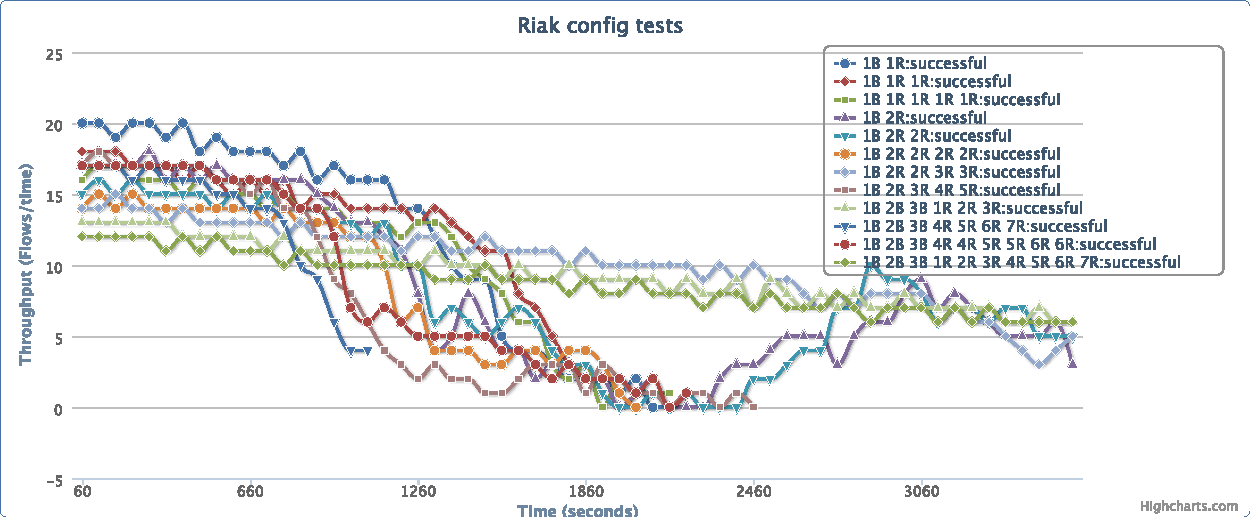
\includegraphics[width=18cm]{./graphics/Load_test-setup.pdf}
 \caption{Load tests of different cluster setups.}
 \label{fig:load_test:setup}
\end{figure}
The x-axis is the time the tests were running and the y-axis the throughput.
The flow included all game play operations like game creation, joining,
order submission and messaging.
Registration and login are not part of it.
The graphs are the different setups, they are labeled with $XR$ or $XB$.
Meaning on machine X there is a {\bf R}iak node or a {\bf B}ackend node
\footnote{1B 2R means there is a backend node on machine 1 and a Riak node on machine 2.}.

As you can see most of them performed quite bad.
Fig.~\ref{fig:load_test:setup2} shows only the best setups.
\begin{figure}[htbp!]
 \hspace{-2.5cm}
 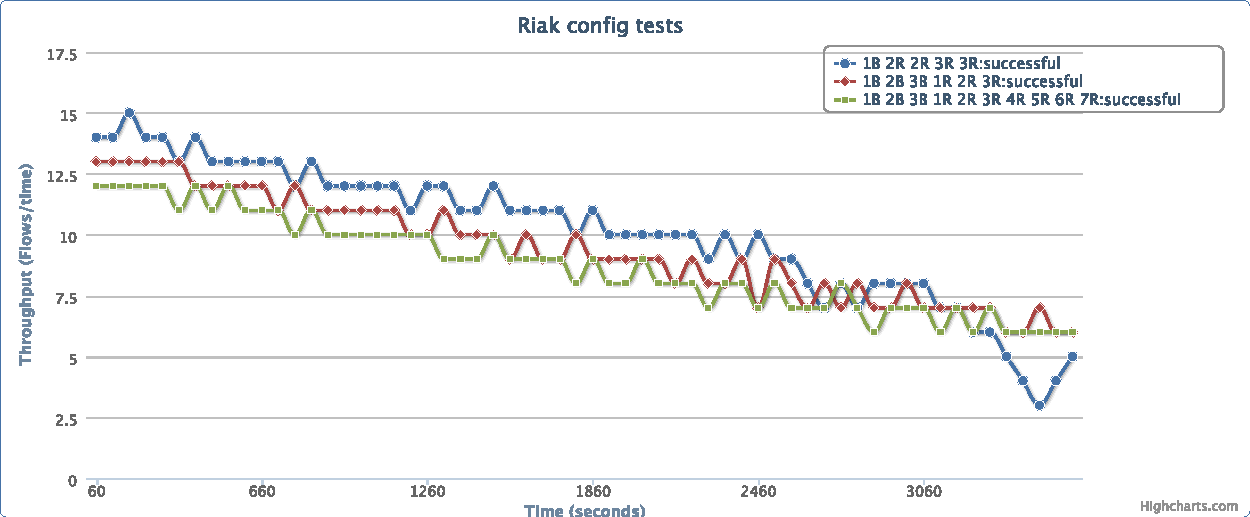
\includegraphics[width=18cm]{./graphics/Load_test-setup2.pdf}
 \caption{The best graphs from Fig.~\ref{fig:load_test:setup}.}
 \label{fig:load_test:setup2}
\end{figure}
These three setups performed more or less the same.
One of these setups is a cluster consisting of three machines each with a Riak and a backend node.
Since this is also the simplest setup we decided to use setups with X machines
each having a a Riak and a backend node in the future.


\subsubsection{Degradation}
The major issue with the previous results was the obvious performance degradation over time.
\begin{figure}[htbp!]
 \hspace{-2.5cm}
 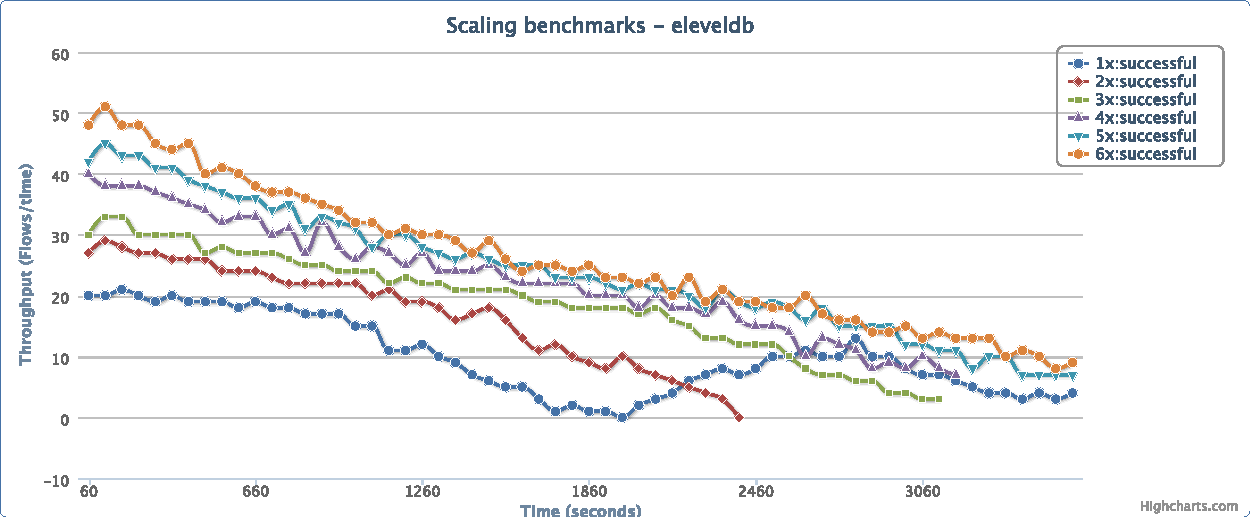
\includegraphics[width=18cm]{./graphics/Load_test-degradation.pdf}
 \caption{Load tests for 1-6 machines.}
 \label{fig:load_test:degradation}
\end{figure}
Fig.~\ref{fig:load_test:degradation} shows that this occured for any cluster size
Preliminary prototype benchmarks did not show this pattern,
which made us compare our system and the prototype we benchmarked.
The main difference was the usage of eLevelDB as Riaks backend storage in the system,
whereas the prototype used bitcask, the default storage backend.

The only reason we used eLevelDB was it being the only backend supporting secondary indices.
We decided to do a comparison of those two backends,
which required to remove the usage of secondary indices.
Therefore we replaced it with Riak search.
As you can see in Fig.~\ref{fig:load_test:degradation_compare} our assumption proved to be correct.
\begin{figure}[htbp!]
 \hspace{-2.5cm}
 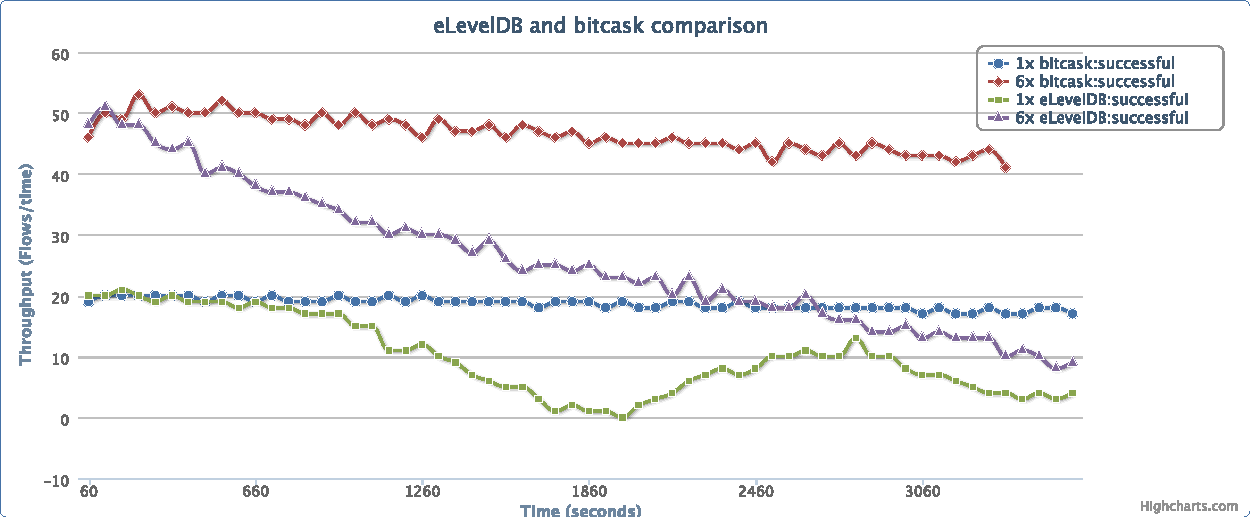
\includegraphics[width=18cm]{./graphics/Load_test-degradation_compare.pdf}
 \caption{Comparison of the storage backends bitcaks and eLevelDB.}
 \label{fig:load_test:degradation_compare}
\end{figure}
Both start of the same but the throughput of eLevelDB version drops quickly,
whereas the bitcask version remains almost stable.

\subsubsection{CAP controls}
Another small but effective change was the adaptation of the Riak CAP controls.
\begin{figure}[htbp!]
 \hspace{-2.5cm}
 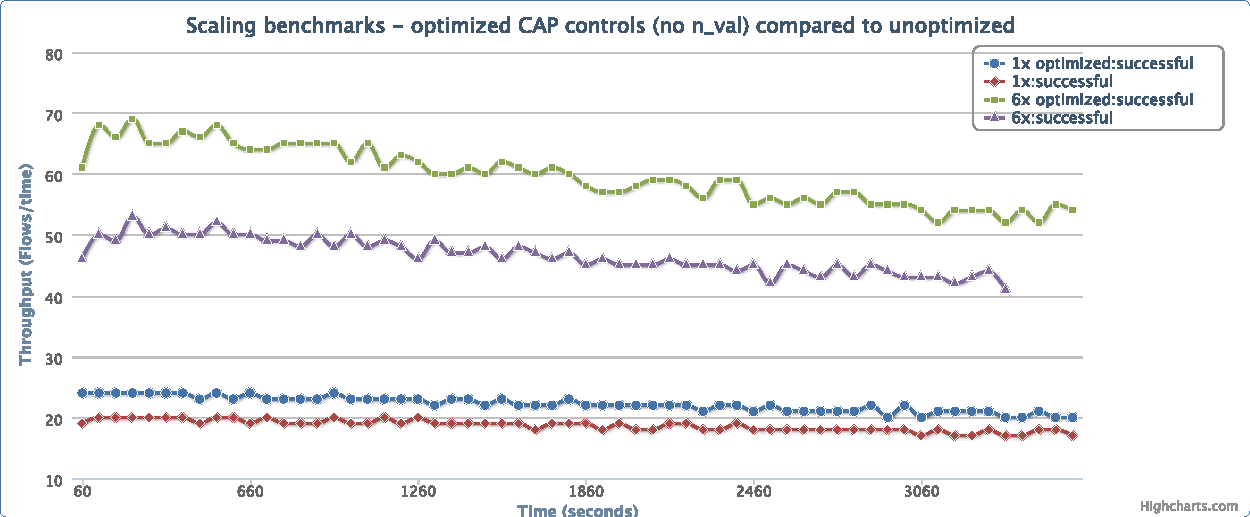
\includegraphics[width=18cm]{./graphics/Load_test-cap.pdf}
 \caption{Improvement by changed CAP controls.}
 \label{fig:load_test:cap}
\end{figure}
Many writes to Riak have a quite low priority.
The message logging for example is such a case.
The system does not need to await confirmation of the write.
Fig.~\ref{fig:load_test:cap} displays the increase in throughput this gave to our system.


\subsubsection{Key filtering}
\label{sec:load_tests:key_filtering}
Despite those improvements the system did still not scale as well as hoped.
The Riak community\footnote{IRC channel \#riak on freenode.net} recommended
us to take a closer look into our Riak search usage,
since it has not been as well tested as other parts of Riak.

The system used Riak search quite extensively, especially after the change from eLevelDB.
In many parts of the system it just replaced secondary indices.
The full text search was not really necessary, as we just needed to find values
without knowing the unique id.
Therefore we tried to replace Riak search in parts with Riaks key filtering.
For messages for example we introduced keys of the form $<unique-id>-<from>-<to>$.
With key filtering it is then possible to query the messages for a certain user without
the use of Riak search.

The advice from the Riak community turned out to be very valuable.
Riak search should be avoided for values that are being written often,
as the indexing is too expensive to scale well.
Unfortunately though we no longer have the data to show a comparison graph.


\subsubsection{Final results}
Fig.~\ref{fig:load_test:scaling} shows the performance of the final system.
\begin{figure}[htbp!]
  \hspace{.5cm}
 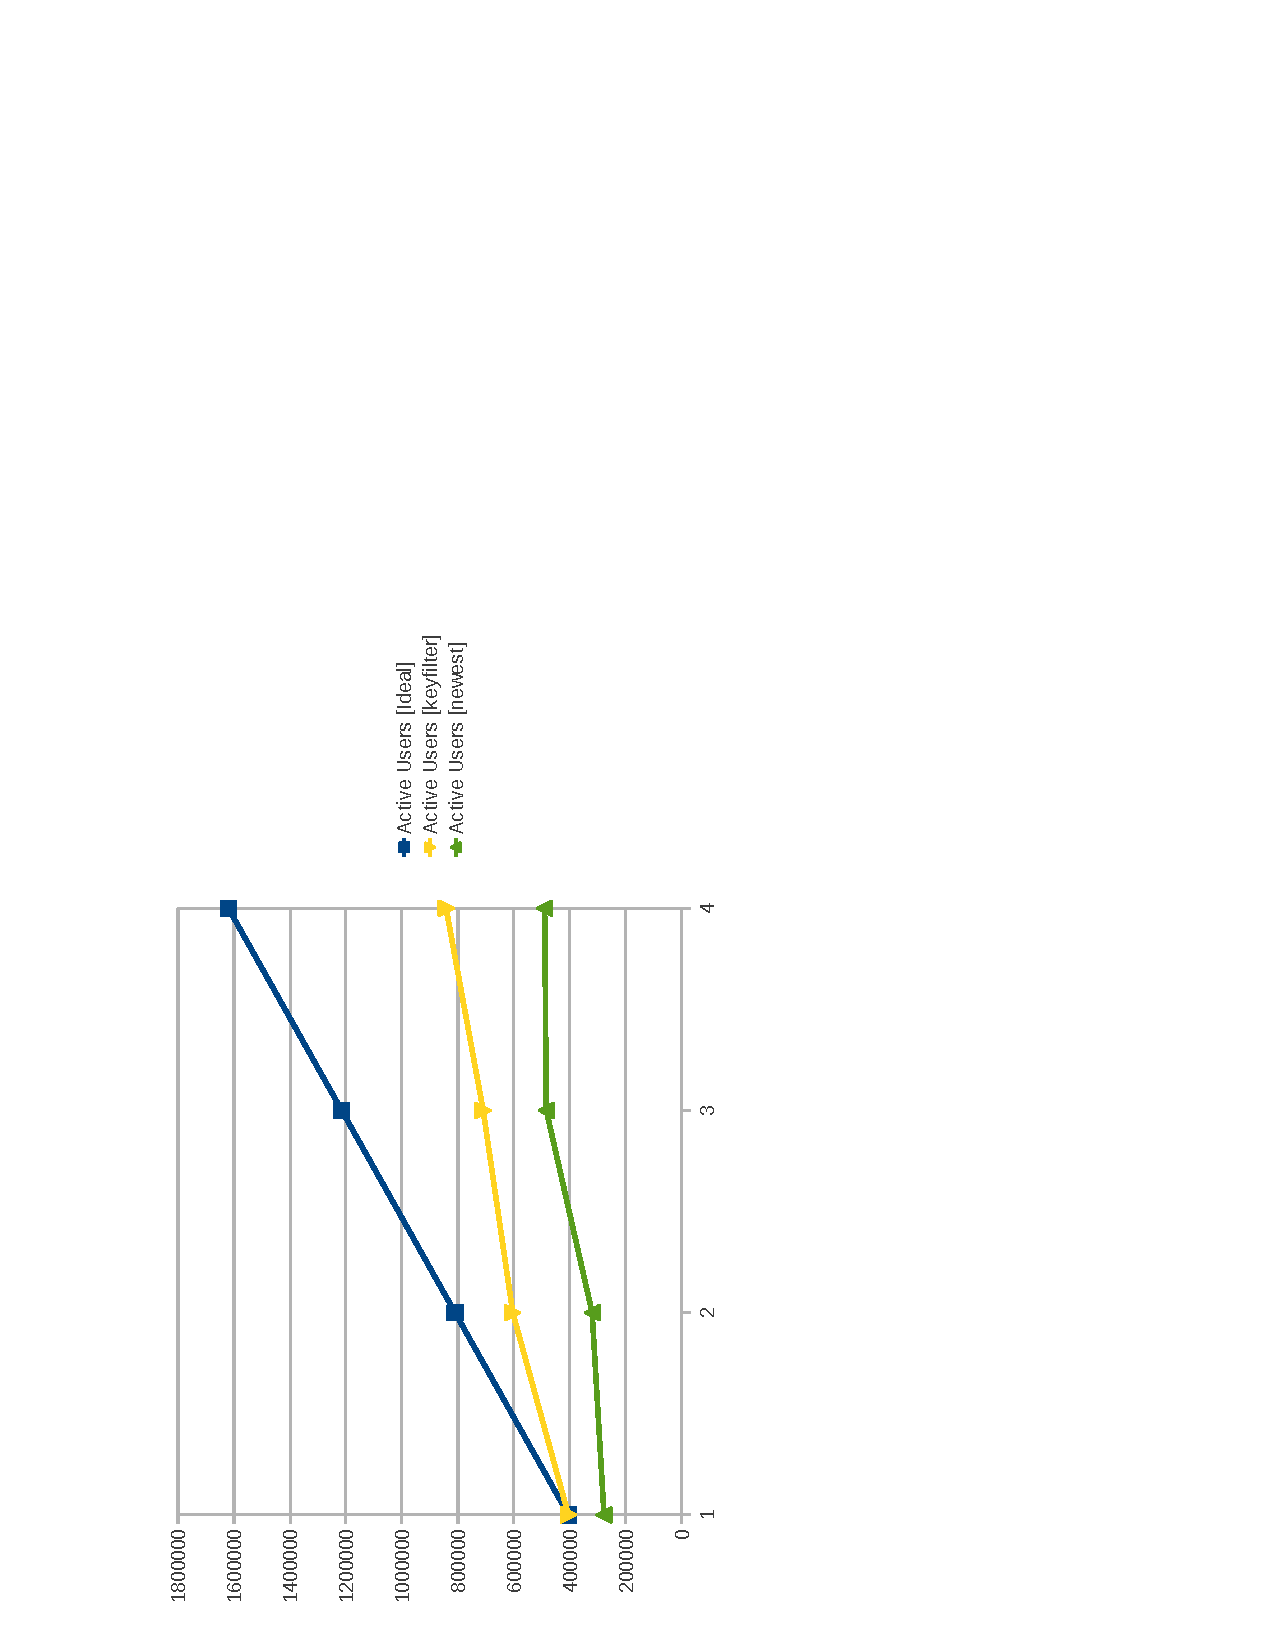
\includegraphics[width=14cm, angle=-90]{./graphics/Load_test-scaling.pdf}
 \vspace{-6cm}
 \caption{Scaling.}
 \label{fig:load_test:scaling}
\end{figure}
The y-axis is the amount of model users the system can handle.
Where a model user is assumed to perform about 20 requests a day and
all users are distributed evenly throughout the day.
The blue one is just for comparison and displays how perfect linear scaling would look like.
The yellow graph shows the performance of the system right after we switched from
riak search to key filtering.
With one machine it can handle around 400k model users, and with 4 machines
a bit more than double the amount.
The green one is the system at the end of this project.

Unfortunately the performance dropped a lot.
The cause for this is a single commit that introduced an increased usage of riak search again.
Unfortunately there was no time left to get the system back to its previous performance.
Still the system performs quite well and 400k model users is most likely
more than the global count of diplomacy players.


\section{Failure Tests}
Our failure tolerance test starts up a cluster of two backends A and B and
starts a game. The basic backend test interacts only via the Web Frontend
for realism but simulates unexpected node or hardware failure by calling
{\tt erlang:halt()} on the relevant backend node.

Since we do not know on which backend the game has been started, we halt
backend~A. If fault tolerance works, we can now be sure that the game is on
backend~B (either it was there in the first place or it got restarted there).

We start the backend~A again and then halt backend~B. Now the game gets moved to
backend~A. This way, we can be sure that the game was moved at least once.
If the game continues to run, the test was successful.

Instructions for running this test are in Sec.~\ref{run_fault_tolerance}.

\chapter{Related Work}
%\hi{Similarities with existing products/systems. How are you similar and how are you different? What do you do better? What can you learn from what's already out there?

%It is possible that you want to have this section earlier, before the system description, perhaps as a part of (the end of) the product description, so that you can refer to it later.}

Diplomacy has been around since the 1950s and has been played by email, snail
mail and through web browsers. Obviously, we are not going to compare ourselves
to the snail mail solution where a game host receives letters with move orders
from the players and the players send each other letters.

Noteworthy browser based solutions are:\\

\begin{tabular}{lc}
  page                            & registered users \\
  \url{http://webdiplomacy.net}   & 40613 \\
  \url{http://playdiplomacy.com/} & 6849
\end{tabular}
\\
\\The alternative email solutions seem to have even lower user numbers but
precise details are hard to be found. Please note that the numbers in
the table are about {\em registered\/} users, while our benchmarks are in terms
of {\em active\/} users.

The advantages the existing solutions have, are generally better interfaces:
the existing email systems are a bit easier to use since you reference games by
name and not by a number and there is no session ID handling involved.
These issues would be fixable with reasonable resources though.

They also provide several game modes (from minor changes to starting units to
playing on a world map). We have the code to handle new maps, but we don't have
the map data. Creating those would be an easy but work-intensive task since
you have to specify all provinces, all connections, starting units, and so on.

Our rules are not perfect yet, they are still a bit rough around the edges but
in probably one or two person weeks would work satisfyingly well.
When it comes to load, we see no problem in handling all web diplomacy
players worldwide (email- and browser-based) with one backend-machine and maybe
more extra frontend machines.

So, in short: to fully catch up with the alternatives, we would need to invest
in bug fixing and user interaction.

\chapter{Conclusions and Future Work}
We are very happy with the work we have done and that the product is, even
though the seemingly endless scope, quite close to being ``ready''.

Despite all this, the work left to be done is considerable:
An AI was in the original requirements but was not delivered due to time
constraints.
Bug fixing in the rule engine is necessary. Scalability could be improved by
applying tracing to the cluster which would be lots of interesting work. A more
polished interface, that is more appealing to the eye is something that could
be worked on.

In order to make the game playable by the public, a better system to find and
join games would probably be necessary in the web frontend --- and we would
need to do lots of hallway testing and/or maybe publish an alpha version in
order to collect feedback.

One more thing would be to think a lot about security --- not much thought has
been spent on it yet.

The rule engine does not support multi-fleet convoys yet but they are important
for the game tactics (the classic Italian opening called
``lepanto~opening''~\cite{lepanto} uses it, for instance).
This could be done quite easily in the rule engine.

\appendix
\chapter{Installation Instructions}
\section{Requirements}
Treacherous Talks was developed using Erlang/OTP version R14B03 on Ubuntu 11.04
(AMD64). It has not been tested with other versions of Erlang/OTP or other Linux
distributions. Since some of our dependencies, notably Riak, currently doesn't
support Erlang/OTP R15, we have not been able to test the system under that
version of Erlang/OTP.

Since all Erlang-releated packages in Ubuntu 11.04 are out-of-date, we opted for
compiling and installing Erlang/OTP by hand on our development machines. In
general, we recommend that users do this as well since it is the easiest way to
get all of the required parts of Erlang/OTP installed on your system.

We will not provide you with build instructions for the Erlang/OTP distribution,
but under Ubuntu 11.04 you will most likely need the {\tt make}, {\tt gcc}, {\tt
  perl}, {\tt m4}, {\tt ncurses-dev} and {\tt libssl-dev} packages available
before attempting to build it.

Before you can build Treacherous Talks itself, a few extra libraries and tools
need to be present on your machine: \\

\begin{tabular}{lll}
  Name & Version & Ubuntu package name \\ \hline
  libexpat & $>$ 1.95 & libexpat-dev \\
  libxml   & -        & libxml2-dev \\
  libpam   & -        & libpam0g-dev \\
  git      & -        & git \\
  wget     & -        & wget \\
\end{tabular} \\
\\
There are two deployment options regarding the database Riak: running a
standalone Riak installation or distributing it alongside the Treacherous Talks
release package. Here we assume that you want to distribute Riak along with the
release package. This involves building Riak as a part of the system build
process.

In order to build Riak you will need the GNU C++ compiler ({\tt g++}) installed
and the package {\tt libstdc++6-VERSION-dev} where {\tt VERSION} is the current
version in the package repository (in Ubuntu 11.04 {\tt VERSION} is 4.5). For
some reason there are no generic packages any more in Ubuntu, so you need to
specify the version.
\section{Building}
With all dependencies and required tools in place, building Treacherous Talks
should be straightforward. First you need to get hold of the source code. The
simplest way is probably to download a tarball from Github. Download it from {\tt
  https://github.com/treacheroustalks/Treacherous\-Talks/tarball/master}.  Untar
the file and enter the source code directory.

First we build Riak since we want to distribute it together with the Treacherous
Talks release package. There is support in the Treacherous Talks Makefile for
building Riak, just run {\tt make riak\_release}. This will download, compile
and release Riak. It then moves the release package into the directory {\tt
  system-release} in the top-level source code directory.

Next it's time to build Treacherous Talks. This is done by executing {\tt
  make}. This will invoke the build tool Rebar~\cite{rebar} that is present in the source
code directory. Rebar will download all dependencies and compile everything in
the right order. This step can take a while to complete.

The final two steps after compiling is to make an Erlang release and create a
tarball that contains everything needed to run the system. By executing {\tt
  make release} a release package will be created and placed into the {\tt
  system-release} directory alongside Riak. After this step, we create a tarball
of everything inside that directory with {\tt make tar\_release}. The resulting
tarball is outputted to the {\tt system-release} directory.

\section{Testing}

\subsection{Unit and Integration Tests}

After building, unit and integration tests can be run together using

\begin{Verbatim}
make test
\end{Verbatim}

This is equivalent to running {\tt make unittest inttest}.

\subsection{Node Failure Tolerance Tests}\label{run_fault_tolerance}

An escript~\cite{escript} {\tt fault\_tolerance} is generated when building a full release. This
allows the tests in {\tt ext\_test/fault\_folerance} to be run from the command
line e.g.

\begin{Verbatim}
./system-release/tt/bin/fault_tolerance   tt.config
\end{Verbatim}
where {\tt tt.config} is a cluster configuration file. This requires the same
setup as the Cluster Manager (see~\ref{sec:settingup}) needs for starting a cluster. The
{\tt fault\_tolerance} escript will exit with a non-zero exit status if any tests
failed and outputs debugging information to the console.

\section{Installing from a release tarball}
\label{sec:installing}
The resulting tarball from the build step is self-contained and can be freely
moved to other computers running the same version of the operating system. To
install the system, simply extract the tarball to a location of your choice. As
usual in Unix-like systems, take care to have the ownership of the files setup
correctly so that the user running Riak and Treacherous Talks has the correct
permissions on all directories and files. The simplest is to have the user
executing the program owning the files.

If you intend to allow any part of the system to communicate over privileged
ports, ensure that the user has privileges to do so.
\section{Setting up and starting the System Manager}
\label{sec:settingup}
There is an application called the System Manager in Treacherous Talks. The
purpose of this application is to configure, start and stop Riak and the rest of
the Treacherous Talks system on a single machine. The System Operator uses the
escript called Cluster Manager to interact with a cluster of System Managers via
RPC calls.

\begin{sloppypar}
Before we can start and configure the system we must set up and start the System
Manager itself. There is only one major setting one can change, and that is the
Erlang node name. Enter the directory where the release tarball was extracted.
Edit the file {\tt system-release/tt/etc/nodename.system\_manager} and change
the domain name or ip address as needed (the part after the @-sign). Note that
you must set domain to something externally available if you intend to run the
Cluster Manager on another machine.
\end{sloppypar}

\begin{sloppypar}
When the node name is set, the System Manager is ready to be started. This is
done by proceeding to the directory where the release tarball was extracted and
then executing the command {\tt system-release/tt/bin/system\_manager start} in
a shell.
\end{sloppypar}
\section{Creating a system-wide configuration file}
The main purpose of having both a System Manager and a Cluster Manager is to
simplify the task of configuring and controlling a cluster of nodes running on
different machines. Even if you only run the releases on a single machine, it
simplifies the task of handling the Treacherous Talks system and Riak.

To do this, a single configuration file is used. The file specifies for the
Cluster Manager where the different System Managers are, what releases a single
machine should run and the configuration of such releases. The configuration is
given as a list of host tuples.

Each host tuple describes a host (machine) and contains the domain or ip address
it has, the name of the System Manager and another list of release tuples.

Each release tuple contains a release name (riak, backend, smtp\_frontend,
xmpp\_frontend, web\_frontend), the actual node name for that release and a list
of configuration options. These configuration options correspond exactly to the
ones available in the release configuration file in the {\tt etc} directory of a
release package. Here is a minimal example for running all releases on a single
machine:

\begin{Verbatim}[samepage=true]
[{host, "127.0.0.1", "system_manager",
  [{release, riak, riak,
    [
     {riak_core, [{http, [{"127.0.0.1", 8091}]}]},
     {riak_kv, [{pb_ip, "127.0.0.1"}, {pb_port, 8081}]},
     {riak_search, [{enabled, true}]}
    ]},
   {release, backend, backend,
    [
     {db, [{riak_ip, "127.0.0.1"}, {riak_database_port, 8091},
           {riak_protobuf_port, 8081}]}
    ]},
   {release, smtp_frontend, smtp_frontend, []},
   {release, xmpp_frontend, xmpp_frontend, []},
   {release, web_frontend, web_frontend, []}
  ]}
].
\end{Verbatim}

\begin{sloppypar}
For more information on the available configuration options, please see the
example configuration file in {\tt system\-release/tt/etc/example.config}.
\end{sloppypar}
\section{Using the Cluster Manager}
When the system-wide configuration file is finished, it is time to put it to
use. The Cluster Manager is a small command-line tool (an escript) that reads
the configuration file and connects to running System Managers to enforce the
state given in the configuration file and/or performs a specific action.

The actions performed is controlled by adding switches when invoking the
command. One can use multiple switches to perform more than one action. A short
description of the more common ones follow.

By using the {\tt --setconfig} switch, the Cluster Manager will try to connect
to all specified System Managers and give them the configuration they should
apply. Note that this does not automatically apply the configuration to a
running system. To be able to use the new configuration, the system must be
restarted.

The {\tt --join} switch is intended to be used whenever a Riak node is added to
the cluster. It will make any new Riak nodes join the already present
nodes. This is only necessary when you add a new node, not after stopping or
starting a Riak node.

Finally, the {\tt --start} and {\tt --stop} switches starts and stops the needed
releases, including Riak if that is needed. To see what releases are running and
responding across a cluster, the {\tt--ping} switch comes handy.

\begin{sloppypar}
To run the Cluster Manager, first go to the directory where the release tarball
was extracted and then execute {\tt system-release/tt/bin/cluster\_manager}. You
also need to supply the name of the configuration file to use and the action to
perform.
\end{sloppypar}
\mbox{}\\
Here is an example run of the Cluster Manager:
\begin{verbatim}
$ ./bin/cluster_manager --setconfig --start etc/example.config
update_config on "127.0.0.1" was ok
start_release riak on "127.0.0.1" was ok
start_release backend on "127.0.0.1" was ok
start_release web_frontend on "127.0.0.1" was ok
start_release xmpp_frontend on "127.0.0.1" was ok
start_release smtp_frontend on "127.0.0.1" was ok
informing 'backend@127.0.0.1', result was: ok
$
\end{verbatim}
\section{Running on a non-bundled Riak installation}
There are a few additional things to consider if you want to run Treacherous
Talks on top of an already running Riak installation instead of using the
bundled one.

Some parts of Treacherous Talks are dependent on Riak Search and special search
schemas. These schemas need to be installed on each Riak node in a cluster
before starting the Treacherous Talks system. This is done automatically when
using the bundled Riak instance and configuring it via the Cluster Manager.

When using a non-bundled Riak installation you need to do this yourself. Each
schema in the {\tt system-release/tt/riak} directory must be installed in each
Riak node. Please consult the Riak manual\footnote{http://wiki.basho.com/Riak-Search---Schema.html}
for the exact steps you need to perform to accomplish this.

You can still use the Cluster Manager for configuring backends and frontends in
this scenario. Remove the riak tuple from the example configuration and ensure
that the db application in the backend knows how to connect to an already
installed Riak node. Ensure that Riak is started before the rest of the system
is started.
\chapter{Maintenance Instructions}
\section{Adding a host to a running cluster}
Sometimes the need arise to add another server to an already running
cluster. This is a rather simple operation when using the Cluster Manager.

First, ensure that the system has been properly installed (see
~\ref{sec:installing}) on the new node. Start the System Manager if not already
started on that node. Then add the configuration of the new node to the
system-wide configuration file.

Finally, run the Cluster Manager with the {\tt --setconfig} and {\tt --start}
switches. The result will be that all releases defined in the configuration file
will be started, included any new ones. If a release is already running nothing
will be done to it and it will be reported by the Cluster Manager as {\tt
  \{error, release\_is\_already\_started\}}. This is a harmless message
indicating that nothing was done for that release.
\section{Removing a host from a running cluster}
Removing a server from a running cluster is normally a straightforward
procedure, but a bit more complicated than adding a server. You cannot simply
remove its entries from the system-wide configuration file and then expect the
Cluster Manager to stop it for you since the configuration declares what
\emph{should} be running on the cluster, not the current state of the cluster.

You have three choices for removing a host:
\begin{enumerate}
  \item Restarting the whole cluster.
  \item Stopping the system manually on the specific host.
  \item Creating a special configuration file for stopping a specific host.
\end{enumerate}

The first solution is simple: just remove the host from the configuration file,
stop and start the cluster using the Cluster Manager. Of course, this has the
disadvantage of making the system unavailable for some time.

\begin{sloppypar}
The second solution, stopping the system manually, is a more attractive
solution. To do this, go to the installation directory on the host you want to
remove. For each release running on the host, run the corresponding executable
with the argument {\tt stop}. Example: {\tt system-release/tt/bin/backend
  stop}.
\end{sloppypar}

The third solution is probably the best one, but requires some effort. Copy your
old configuration file before removing the entry describing the host you want to
remove. Remove everything else in the copied configuration file except for the
host you want to remove from the cluster. Now use this configuration when
running Cluster Manager with the {\tt --stop} switch. Only the host you want to
remove has now been stopped.

Nothing else needs to be done for the Treacherous Talks system when removing a
host. Any games running on the now stopped backend will be automatically moved
to other backends.

If you want to remove a Riak node permanently, you should tell the Riak cluster
about it so that it can redistribute the data on that node onto other nodes in
the cluster. Please see the Riak manual\footnote{http://wiki.basho.com/Adding-and-Removing-Nodes.html}
for more information.

\section{System Operator Interface}
Being a system operator opens up a few special features, some are available as
text based commands but all are available in the web interface of the operator:
\begin{itemize}
\item Adding or removing moderators (web only).
\item Stop games (web only).
\item Overview games including moves and messaging (web only).
\item Blacklist or whitelist players.
\item Receive reports about issues from players (web only).
\item Send messages to players in any game.
\item View the status of the system (web only).
\item View the status of Riak.
\end{itemize}

The status of the system gives information about which applications are running
on which nodes, the number of workers they have and information about their
message queue lengths. This can be used to determine the health of the system
and see if an application needs to be started on another node or perhaps if it
could be fixed by increasing/decreasing the number of workers.

\subsection{Moderators}
A moderator is a priviledged user which can access a moderator page in the web
interface.\\

The following features are available for moderators:
\begin{itemize}
\item Blacklist or whitelist players.
\item Send messages to players in any game.
\item Receive reports from players reporting other players (web only).
\end{itemize}

\chapter{Text based commands}
\label{sec:textbasedcommands}

\section{Playing the game}
The web interface is the only one to provide means to interactively select
orders, but it is also possible to give text based orders as through IM and
email.\\

\subsection*{Writing orders}
Alternative ways to write a move order (also used for retreat orders):
\begin{verbatim}
army warsaw move prussia
a war m pru
a war - pru
a war -> pru
\end{verbatim}
Alternative ways to write a convoy order:
\begin{verbatim}
fleet north_atlantic_ocean convoy army london move norwegian_sea
f nth c a lon m nrg
f nth c a lon - nrg
f nth c a lon -> nrg
\end{verbatim}
Alternative ways to write a hold order:
\begin{verbatim}
army london hold
a lon h
\end{verbatim}
Alternative ways to write a support order:
\begin{verbatim}
army galicia support budapest
a dal s a bud
\end{verbatim}
Alternative ways to write a build order:
\begin{verbatim}
build army munich
b a mun
\end{verbatim}
\newpage

\subsection*{List of provinces and water bodies and their abbreviations}
\begin{tabular}{ l | l | l }
adriatic\_sea - adr & aegean\_sea - aeg & albania - alb \\
ankara - ank & apulia - apu & armenia arm \\
baltic\_sea - bal & barents\_sea - bar & belgium - bel \\
berlin - ber & black\_sea - bla & bohemia - boh \\
brest - bre & budapest - bud & bulgaria - bul \\
burgundy - bur & clyde - bly & constantinople - con \\
denmark - den & eastern\_mediterranean - eas & edinburgh - edi \\
english\_channel - eng & finland - fin & galicia - gal \\
gascony - gas & greece - gre & gulf\_of\_bothnia - bot \\
gulf\_of\_lyon - gol & helgoland\_bight - hel & holland - hol \\
ionian\_sea - ion & irish\_sea - iri & kiel - kie \\
liverpool - lvp & livonia - lvn & london - lon \\
marseilles - mar & mid\_atlantic\_ocean - mid & moscow - mos \\
munich - mun & naples - nap & north\_africa - naf \\
north\_atlantic\_ocean - nat & north\_sea - nth & norway - why \\
norwegian\_sea - nrg & paris - par & picardy - pic \\
piedmont - pie & portugal - por & prussia - pru \\
rome - rom & ruhr - ruh & rumania - rum \\
serbia - ser & sevastopol - sev & silesia - sil \\
skagerrak - ska & smyrna - smy & spain - spa \\
st\_petersburg - stp & sweden - swe & syria - syr \\
trieste - tri & tunis - tun & tuscany - tus \\
tyrolia - tyr & tyrrhenian\_sea - tyn & ukraine ukr \\
venice - ven & vienna - vie & wales - wal \\
warsaw - war & western\_mediterranean & yorkshire - yor \\
\end{tabular}

\newpage
\section{Commands for IM and Mail}
\label{sec:textbasedcmd}
The following commands are available for IM and mail users:

\begin{verbatim}
REGISTER
required: NICKNAME, PASSWORD, EMAIL, FULLNAME
optional: CHANNEL

UPDATE
required: SESSION
optional: PASSWORD, EMAIL, FULLNAME

LOGIN
required: NICKNAME, PASSWORD

LOGOUT
required: SESSION

ORDER
required: SESSION, GAMEID

CREATE
required: SESSION, GAMENAME, PRESSTYPE, ORDERCIRCLE,
          RETREATCIRCLE, GAINLOSTCIRCLE, WAITTIME
optional: PASSWORD, DESCRIPTION, NUMBEROFPLAYERS

RECONFIG
required: SESSION, GAMEID
optional: GAMENAME, PRESSTYPE, ORDERCIRCLE, RETREATCIRCLE,
          GAINLOSTCIRCLE, WAITTIME, PASSWORD, DESCRIPTION,
          NUMBEROFPLAYERS

OVERVIEW
required: SESSION, GAMEID

VIEWCURRENTGAMES
required: SESSION

JOIN
required: SESSION, GAMEID, COUNTRY

SEARCH
required: SESSION
optional: GAMEID, GAMENAME, DESCRIPTION, PRESSTYPE, STATUS,
          ORDERCIRCLE, RETREATCIRCLE, GAINLOSTCIRCLE,
          WAITTIME, NUMBEROFPLAYERS

MESSAGE (in game messages)
required: SESSION, GAMEID, CONTENT
optional: TO

MESSAGE (out of game messages)
required: SESSION, TO, CONTENT

GETPROFILE
required: SESSION

GETPRESENCE
required: SESSION, NICKNAME

REPORTPLAYER
required: SESSION, CONTENT

REPORTISSUE
required: SESSION, CONTENT


MODERATOR and OPERATOR only commands:

POWERMESSAGE
required: SESSION, GAMEID, CONTENT
optional: TO

BLACKLIST
required: SESSION, NICKNAME

WHITELIST
required: SESSION, NICKNAME

\end{verbatim}


The general format to send any command is
\begin{verbatim}
COMMAND
FIELD: <data>
END
\end{verbatim}

where \verb|FIELD| is the name of the field and \verb|<data>| is the
input from the user, \emph{all commands and fieldnames must be in capital
letters}.


\subsection*{Example commands}
\label{sec:examplecmd}
\begin{verbatim}
REGISTER
NICKNAME: bob
PASSWORD: secret
EMAIL: bob@email.com
FULLNAME: Bob Cat
END

MESSAGE
SESSION: g2dkABFiYWNrZW5kQDEyNy4wLjAuMQAAA+QAAAAAAQ==
GAMEID: 12345
TO: england, france
CONTENT:
Hi! Would you like to help me take down russia?
END
\end{verbatim}

Order writing is done as in the previous section, as content for the
\verb|ORDER| command:
\begin{verbatim}
ORDER
SESSION: g2dkABFiYWNrZW5kQDEyNy4wLjAuMQAAA+QAAAAAAQ==
GAMEID: 12345

army ven -> tri
army tyr support a ven -> tri
END
\end{verbatim}

\renewcommand\bibname{References}
\bibliographystyle{unsrtnat}
\bibliography{product_rep}

\end{document}
